\documentclass[12pt,letterpaper]{article}

\usepackage{xcolor}
\usepackage{fontspec}
\usepackage{tipa}
\usepackage{amssymb}
\usepackage{booktabs}
\usepackage{microtype}

\usepackage{tikz}
\usetikzlibrary{arrows.meta,shapes,positioning,fit,backgrounds}
\usepackage{pgfplots}
\pgfplotsset{compat=1.18}



\usepackage[style=langsci-unified,backend=biber]{biblatex}
\addbibresource{refs.bib}

% Define the missing colors
\definecolor{lsLightBlue}{RGB}{201,233,246}
\definecolor{lsMidBlue}{RGB}{0,114,178}
\definecolor{lsDarkBlue}{RGB}{0,62,110}
\definecolor{lsLightGreen}{RGB}{181,226,140}
\definecolor{lsMidGreen}{RGB}{97,163,65}
\definecolor{lsDarkGreen}{RGB}{0,116,0}
\definecolor{lsLightOrange}{RGB}{255,229,204}
\definecolor{lsMidOrange}{RGB}{255,117,0}
\definecolor{lsDarkOrange}{RGB}{193,89,0}
\definecolor{lsLightGray}{RGB}{240,240,240}
\definecolor{lsMidGray}{RGB}{180,180,180}
\definecolor{lsDarkGray}{RGB}{77,77,77}
\definecolor{lsNightBlue}{RGB}{0,49,80}
\definecolor{lsNightGreen}{RGB}{0,75,0}
\definecolor{lsNightOrange}{RGB}{154,77,0}
\definecolor{lsDOIGray}{RGB}{80,80,80}

\usepackage{csquotes}
\usepackage{langsci-gb4e}
\usepackage{hyperref}
\hypersetup{
    colorlinks=true,
    linkcolor=blue,
    filecolor=magenta,
    citecolor=blue,    
    urlcolor=cyan,
    pdftitle={Grammaticality de-idealized},
}
\usepackage[normalem]{ulem}
\usepackage{orcidlink}
\usepackage{authblk}
\usepackage{amsmath}
\usepackage{rotating}


% Redefine page number format in citations
\DeclareFieldFormat{postnote}{#1}
\DeclareFieldFormat{multipostnote}{#1}

\title{Grammaticality de-idealized}

\author{Brett Reynolds}
\date{\today}

\begin{document}
\maketitle

\begin{abstract}
    This paper introduces a novel theoretical framework for (un)gram\-maticality, distinct from traditional grammars focused solely on language production or description. The proposed model conceptualizes (un)grammaticality explicitly as coherence in form–meaning pairings accepted or rejected by language communities, integrating morphosyntactic, semantic–pragmatic, and social dimensions. Previous approaches, including generative grammar, Construction Grammar, and psycholinguistic models, have not adequately explained why grammaticality is specifically restricted to morphosyntax, why semantically coherent constructions may nonetheless be deemed ungrammatical, or why certain semantically transparent structures remain systematically blocked. The present framework addresses these gaps by providing a principled explanation of (un)grammaticality rooted in community standards for communicative coherence, rather than relying exclusively on structural or intuition-based definitions.
\end{abstract}

Report: https://chatgpt.com/share/68498638-5d38-8009-94ca-7007915fe08a

\newpage
\section*{Introduction}

Every competent speaker of English knows that *\textit{Can the have running} is impossible, but the source of this certainty proves remarkably elusive. What do we mean when we say a sentence is ungrammatical? Consider these examples:

\ea \label{ex:starting-stars}
\ea\label{ex:nonsense} *\textit{Can the have running?}
\ex\label{ex:tense} *\textit{I've finished it yesterday.}
\ex\textsuperscript{?}\textit{I saw Joan, a friend of whose was visiting.}\label{ex:whose} 
\ex\label{ex:center} \textit{~The bread the baker the apprentice helped made is delicious.}
\ex\label{ex:age} \textbf{~A:} \textit{~How old are you?} \textbf{B:} *\textit{I have 25 years.}
\ex\label{ex:lbe} *\textit{Which did you buy car?}
\z\z

While all might receive asterisks in many analyses, they represent fundamentally different types of unacceptability. Some constructions, like (\ref{ex:nonsense}), fail to pair form with any meaning in English. Others, like (\ref{ex:tense}), involve a clash between the time semantics of clause tense and the word \textit{yesterday}. Still others, such as (\ref{ex:whose}) show gradient or indeterminate status. (\ref{ex:center}) illustrates what we might call theoretically predicted acceptability~-- constructions that linguistic theory predicts should be grammatical but are consistently rejected by native speakers. Still others, like (\ref{ex:age}) are grammatical in some contexts but not others. And a few, like the left-branch extraction of (\ref{ex:lbe}), seem to be ruled out entirely, despite being apparently short and interpretable.

Different theoretical traditions have emphasized different aspects of grammaticality: formal approaches focus on abstract principles, usage-based theories stress frequency and entrenchment, and processing accounts highlight cognitive constraints. But we still lack a unified framework that can explain both categorical blocks and gradient acceptability while accounting for cross-linguistic variation and change over time.

This paper presents such a framework, building on insights from both generative and functional traditions to propose that grammaticality should be understood in terms of form--meaning pairings that evolve within specific language communities. These pairings interact with both universal processing constraints and sociolinguistic factors to produce the complex patterns of acceptability we observe in actual language use. The framework rests on three key premises:

\begin{enumerate}
\item At its core, grammaticality involves conventional form--meaning pairings within specific language communities, dialects, registers, and situations.
\item These pairings interact systematically with processing constraints, sociolinguistic factors, and other linguistic subsystems (phonology, semantics, pragmatics).
\item Grammaticality reflects the degree to which an utterance establishes stable, community-recognized form-meaning pairings. Various factors can disrupt this stability~-- from complete absence of conventional pairings to conflicts between competing interpretations~-- producing a spectrum of ungrammaticality effects that share the core property of form-meaning instability.
\end{enumerate}

These premises directly address key limitations in previous approaches to grammaticality. The first premise moves beyond the abstract competence model of early generative grammar while while building upon its analyses of systematic constraints. It provides a theoretical foundation for explaining both categorical blocks like (\ref{ex:lbe}) and gradient acceptability like (\ref{ex:whose}), aligning with Francis's \autocite{francis2022} arguments for incorporating gradience into core grammatical theory. The second premise resolves a long-standing tension between formal syntactic approaches and processing-based accounts by explicitly modelling their interaction rather than treating them as competing explanations. This allows us to explain why some ungrammatical constructions resist improvement through exposure while others become more acceptable with familiarity. The third premise provides a principled basis for phenomena that have resisted unified explanation in both generative and functional frameworks.

The paper proceeds as follows. Section \ref{sec:previous} examines the impasse in grammaticality theory, tracing how different theoretical traditions~-- from early generative grammar through contemporary experimental approaches~-- have attempted to reconcile form, meaning, and acceptability. Section \ref{sec:framework} presents the framework in detail, identifying twelve key principles that govern grammaticality and grammaticality judgments. Section \ref{sec:formalism} presents a simple formal model that illustrates how the framework's key components interact to produce grammaticality judgments. Section \ref{sec:implications} explores the theoretical implications of this approach, particularly its relationship to generative grammar, Construction Grammar, and usage-based theories, and includes specific predictions about cross-linguistic variation in grammaticality judgments and the conditions under which satiation effects should occur. The paper concludes by acknowledging limitations of the current framework and suggesting directions for future research using corpus analysis, experimental methods, and cross-linguistic investigation.

\section{The Impasse in Grammaticality Theory}\label{sec:previous}

The concept of grammaticality remains elusive despite its centrality to linguistic theory. After decades of research, we still lack a comprehensive account of what makes an utterance grammatical or ungrammatical. This theoretical impasse stems from three fundamental tensions in how grammaticality has been conceptualized.

First, there is the tension between categorical rules and gradient judgments. \textcite{chomsky1957}, building on formal production systems developed by \textcite{post1943}, treated grammaticality as a categorical property defined by membership in a set of well-formed strings. This approach yielded important insights into systematic constraints and hierarchical structure, but struggled with empirical evidence showing that speakers consistently provide gradient judgments. The competence-performance distinction introduced by \textcite{chomsky1965} attempted to preserve categorical grammar by attributing gradience to processing limitations rather than grammatical knowledge itself. Yet as \textcite[71]{schutze2016} notes, this allows results that support the theory to count as evidence while contrary results are \enquote{dismissed as performance artifacts.} Consider center-embedded relatives like (\ref{ex:center}) \textit{The bread the baker the apprentice helped made is delicious}, which many theories classify as \enquote{grammatical but unprocessable.} This classification doesn't explain why these structures feel ungrammatical to speakers; it merely restates the problem in different terms.

Second, there is the tension between form and meaning in grammaticality. Chomsky's famous example (\ref{ex:colorless-grammatica}) was intended to demonstrate that syntax operates independently from semantics. But many grammaticality judgments clearly depend on meaning. When speakers reject (\ref{ex:tense}) \textit{*I've finished it yesterday}, they're responding to a clash between the present perfect's current relevance meaning and the adverb's completed past meaning. Generative semanticists like \textcite{lakoff1971} and \textcite{mccawley1968} demonstrated that many seemingly syntactic constraints have semantic motivations. \textcite{morgan1973} showed that contextual factors can dramatically alter judgments: \textit{Spiro conjectures Ex-Lax} becomes perfectly acceptable as an answer to \textit{Does anyone know what Mrs. Nixon frosts her cakes with?} Construction Grammar \autocite{goldberg1995constructions} has productively integrated form and meaning, showing how constructions carry meanings that interact with lexical semantics. This perspective helps explain why novel uses that align with established constructional meanings (like \textit{She texted him the address}) are accepted, while those that clash with constructional semantics (like \textit{*She disappeared him the evidence}) are rejected.

Third, there is the tension between universal principles and community conventions. Sociolinguistic research \autocite{labov1972} has demonstrated that grammaticality must reference community norms rather than universal principles alone. Cross-linguistic variation in grammatical patterns shows that each language community conventionalizes particular form--meaning mappings through historical processes. These conventions become entrenched through statistical preemption \autocite{Goldberg2011}~-- speakers learn that certain forms are ungrammatical precisely because they encounter alternative expressions in contexts where the ungrammatical form would otherwise be expected. Usage-based approaches \autocite{bybee2006} have emphasized that grammatical knowledge emerges from patterns of language use, but haven't fully explained why certain extremely rare constructions remain grammatical while other, more frequent patterns trigger ungrammaticality judgments. (see Author (in prep.) for an evolutionary account of the attentional bias that supplies the relevant input statistics.)

These tensions have created a landscape where each framework captures important aspects of grammaticality but none provides a comprehensive account. Experimental approaches have improved methodological rigour but sometimes mistake measurement for explanation. As \textcite{schutze2016} reminds us, acceptability judgments are behavioural measures that require theoretical interpretation. What's needed is not another taxonomic classification of grammaticality types, but rather a framework that explains why grammaticality judgments pattern as they do across languages and communities.

\section{The Morphosyntactic-Meaning Model of Grammaticality}\label{sec:framework}

This section presents the proposed MMMG framework, organizing the account around six core components that interact to determine grammaticality, followed by analysis of the patterns these interactions produce and the mechanisms driving change over time.

\subsection{Core Components of Grammaticality}\label{sec:core-components}

The framework identifies six causally interpretable dimensions that interact to determine whether a construction is grammatical within a given communicative context. These components represent the fundamental building blocks from which grammaticality emerges.

\subsubsection{Morphosyntactic form--meaning pairings within communities}\label{sec:f-m-pair-in-community}

At its foundation, grammaticality depends on the existence of stable pairings between morphosyntactic forms and their meanings within specific language communities. This component encompasses both the basic insight that forms carry meaning and the observation that different communities conventionalize different form--meaning relationships.

\paragraph{Form--meaning pairings}

That forms are inherently meaningful~-- syntactic and morphological forms just as much as words~-- is a key tenet of Construction Grammar. And just as words tend to be polysemous, typically having a core sense that is overwhelmingly more common than all others \autocite{Kilgarriff2004}, so too do morphosyntactic forms. For instance, the English past tense usually means past time, but it can also denote deference/social distance as in (\textit{Could you?}) or a low level of likelihood (\textit{If I went \dots}).

A construction like that instantiated by \textit{old men} is a bare plural construction. Setting aside its lexical semantics, we can think about the meaning of its form like this: In English, a bare plural often denotes a category or kind, rather than a specific, individuated set or token. The adjective \textit{old} is a pre-head modifier attached to \textit{men}, contributing a property (advanced age) attributed to the head noun (adult male humans).

But the same construction instantiated by \textit{other men} shows how a single construction type can accommodate different form--meaning relationships. While both strings share the same surface syntax of [Modifier:AdjP Head:NP-\textsc{pl}], \textit{old} contributes a property that directly modifies the noun's denotation, while \textit{other} establishes a complementary relation, requiring a contextually salient reference set of men and defining its denotation in terms of non-membership in that set. This illustrates how the pre-nominal modifier construction, like the past-tense form discussed above, can encode quite different meanings. In sum, forms have meanings and are usually polysemous.

Neuroimaging studies from Ev Fedorenko and her collaborators, using fMRI and functional localization techniques, offer evidence for the close relationship between syntactic and semantic processing \autocite{Fedorenko2011, Fedorenko2012, Fedorenko2024}. Their ``language localizer'' consistently identifies a network of brain regions in the frontal and temporal lobes that show significantly higher activation during language tasks than during non-language tasks \autocite{Fedorenko2010,}. This language network responds to both syntactic and semantic manipulations, suggesting a shared neural substrate for processing both structure and meaning. This aligns with the MMMG's assertion that morphosyntactic form and meaning are deeply intertwined within specific language communities.

\paragraph{Community-specific conventions}

Grammaticality emerges from regularities that hold within a particular language community, dialect, register, or situation, or what \textcite[3]{wiese2023} calls a ``communicative-situation''.

These ``com-sits'' are neither static nor mutually exclusive. A speaker may simultaneously participate in multiple overlapping communities (professional, regional, generational), each with its own grammatical conventions. And these communities evolve over time as speakers join or leave them, as communicative needs change, and as social dynamics shift. This fluidity, rather than undermining the role of community in grammaticality, helps explain phenomena like style-shifting, the emergence of new dialects, and the gradual acceptance of initially marginal constructions. What matters for grammaticality is not the permanence of any particular community but rather the stability of form--meaning pairings within whatever constellation of communities is relevant to a given communicative situation.

This is visible in early child language, where toddlers produce utterances that deviate from adult norms but remain internally consistent within the child's developing system. A toddler in a monolingual English household might say:

\ea
\textit{Ava cookie.} (intended as `Ava = I want a cookie')
\z
Although this differs from adult English norms, it may not be perceived as ungrammatical by the child's regular caregivers. Used with the same pragmasemantic force among anglophone adults, the construction would be judged ungrammatical.

Multiple modal constructions provide another clear example of community-relative grammaticality:

\ea
\textit{I might could help you with that.}
\z
This combination of modal auxiliaries is systematically possible for some American English speakers, who can productively generate similar constructions \autocite{morin2024semantics}. Speakers from communities where only single modals are grammatical, though, typically reject such combinations as ungrammatical.

A similar dynamic appears in code-mixing among bilingual speakers, where combinations of forms from different languages can be grammatical within that bilingual community's norms but not without. Consider a Spanish-English bilingual speaker who uses a Spanish progressive auxiliary with an English lexical verb:

\ea[]{
\gll \textit{Ayer}, \textit{estábamos} \textit{lifting} \textit{en} \textit{el} \textit{gym} \textit{durante} \textit{una} \textit{hora.}\\
yesterday be.\textsc{impf-1pl} lifting in the gym for an hour\\
\glt `Yesterday, we were lifting in the gym for an hour.'} \label{ex:estábamos-lifting}
\z
Within the right communicative situation, this utterance is grammatical. The Spanish auxiliary \textit{estábamos} combines with an English participial form \textit{lifting} to form the progressive aspect. This cross-linguistic pairing of morphology and a lexical verb is consistent with local norms, where code-mixed utterances are common and meaningful. In contrast, a standard monolingual Spanish community, which expects fully Spanish progressive structures (\textit{estábamos levantando pesas}), may judge the example in (\ref{ex:estábamos-lifting}) as ungrammatical. The use of intransitive \textit{lifting}, specific to the gym community, further illustrates just how localized grammaticality judgments can be.

This doesn't mean bilingual communities simply accept any combination of languages. As Toribio (2001) reports, Spanish--English bilingual speakers judge examples like (\ref{ex:enanitos-failed}) as unacceptable, showing that even in bilingual communities, there are systematic constraints on which language combinations are permitted.

\ea[*]{
\gll \textit{Los} \textit{enanitos} \textit{intentaron} \textit{pero} \textit{no} \textit{succeeded} \textit{in} \textit{awakening} \textit{Snow} \textit{White} \autocite{Toribio2001}\\
the dwarfs try.\textsc{pst-3pl} but not succeeded in awakening Snow White\\
\glt `The dwarfs tried but did not succeed in awakening Snow White.'}\label{ex:enanitos-failed}
\z

In a slightly different case, as a second-language speaker of Japanese, I used to say
\ea[*]{\gll \textit{Kawaii} \textit{da}.\\
cute-\textsc{pres} \textsc{cop.pres}\\
\glt `(That)'s cute.' (intended)}
\z
Conventionally, though, the redundant tense marking has no accepted meaning, making the use of the copula ungrammatical to most Japanese speakers, though it felt meaningful and grammatical to me. The example underscores that stable form--meaning pairings emerge from and depend on the shared linguistic routines of a particular community, and individuals with differing trajectories of acquisition may diverge in their grammatical judgments.

The specific linguistic context can matter too. ``To take an obvious case which Jerry Morgan [(\citeyear{morgan1973})] discussed recently, certain combinations of words are extremely strange if presented in isolation but are perfectly normal as answers to certain questions. \textit{Spiro conjectures Ex-Lax} would generally be felt to be unintelligible if presented out of context but is a perfectly normal answer to the question \textit{Does anyone know what Mrs. Nixon frosts her cakes with?}'' \autocite[252, italics added]{McCawley1974}.\footnote{The humour derives from political tensions of the Watergate era, when both Vice-President Spiro Agnew and President Nixon would ultimately resign from office.}

These examples illustrate how each language community, dialect, register, and situation defines its own grammaticality conditions. A form that is grammatical in one communicative situation may be ungrammatical when viewed from the perspective of another. The facts of grammaticality can also diverge for conversants from different communities. This divergence arises because grammaticality is community- and situation-relative: the same utterance can be fully grammatical for those who share the relevant background and ungrammatical for those who don't. The linguist's task is therefore to determine whether a form is grammatical for any language community, or systematically excluded across all.

The stability of form--meaning pairings within speech communities can be empirically modelled, as demonstrated by \textcite{blythe2009speech}. Their utterance selection model treats speech communities as networks where speakers track and reproduce linguistic variants based on their interactions. When applied to dialect formation, these models show how competing linguistic variants spread and eventually stabilize, with initial variant frequency strongly predicting which form will prevail.

\paragraph{Community values and grammatical distinctions}

Different language communities encode different distinctions as grammatically obligatory, reflecting what each community deems relevant enough to systematically mark. Over time, communities establish patterns~-- grammatical constructions~-- that reliably signal these chosen distinctions. As a result, what counts as a grammatical necessity in one language may be optional or absent in another.

The progressive aspect provides a useful example. In English, it's not merely an option but an obligatory grammatical marker for ongoing, incomplete actions:
\ea
\textit{She is studying right now.}
\z
Here, the progressive form \textit{is studying} isn't just a stylistic choice. it's the recognized, grammatical way to express a currently unfolding activity. English speakers strongly prefer (and in many contexts, demand) the progressive construction to convey immediacy and ongoingness.

French, by contrast, doesn't treat the progressive aspect as a grammatically mandatory distinction. While one can signal ongoing activity through adverbs or periphrastic constructions, standard French doesn't have a dedicated progressive form. The sentence:
\ea
\textit{Elle étudie maintenant.}\\
`she studies/is studying now'
\z
can comfortably describe a currently ongoing action without any need for special morphology. The community hasn't defined this aspectual distinction as something requiring marked morphosyntax. What is grammatically necessary in English~-- employing the progressive to signal ongoingness~-- is simply not a requirement in French.

A similar dynamic emerges with evidentiality, the grammatical marking of information sources. In Turkish, evidentiality is systematically encoded through verb forms and particles that distinguish between directly witnessed events and those inferred or reported:
\ea
\textit{Gelmiş}\\
`He/she came (apparently)' \\(i.e., the speaker wasn't a witness but inferred or heard about it.)
\z
The language community treats evidential distinctions as central enough to be baked into the grammar. A speaker can't simply omit evidential marking without sounding ungrammatical.

Needless to say that, while English speakers can say \textit{I heard that he arrived} or \textit{He must have arrived}, these are optional lexical or modal resources rather than required elements of the grammar. The English community simply doesn't regard evidential distinctions as something that must always be encoded morphosyntactically.

\textcite{kilani2005} demonstrate this principle systematically in their analysis of verbal morphology across French and other Romance languages. They show how apparently similar verbal systems can encode quite different semantic distinctions as grammatically obligatory, reflecting each community's conventions about which meaning distinctions must be systematically marked. For instance, while both French and Italian mark aspect morphologically, they differ in which aspectual distinctions are grammaticalized versus left to optional lexical expression.

\paragraph{Why further layers are necessary}
Establishing a form--meaning mapping is a prerequisite for grammaticality, but it isn't sufficient. Individuals routinely interpret strings that the community nevertheless judges ill-formed. That very flexibility forces the grammar to police \emph{how} a pairing is licensed, not merely \emph{whether} one can be imagined in principle. In other words, the system needs additional filters that (i) rule out mappings that conflict with conventional constructional meanings (\S\ref{sec:semantic-compatibility}), (ii) flag mappings whose recovery cost overwhelms processing resources (\S\ref{sec:processing-constraints}), and (iii) block mappings the community has never ratified (\S\ref{sec:community-acceptance}). Only by layering these constraints on top of the initial pairing do we predict the empirical fact that *\textit{Furiously sleep ideas green colorless} elicits universal rejection while (\ref{ex:center}) feels bad in everyday quotation yet is accepted as “grammatical but hard to process’’ once speakers are walked through the intended parse. The extra layers therefore partition the wide space of imaginable pairings into the much smaller subset that a community recognizes as bona fide grammatical resources.

One might object that the community’s verdict alone should settle the matter: if speakers converge on using a form, why not define $G(u)$ as simply `whatever the community accepts'? That move is circular and empirically empty: it can neither flag emerging innovations whose status is still contested nor explain why stable dialectal differences persist despite mutual intelligibility. A purely sociological definition would also mis-classify well-attested performance errors (e.g.\ agreement slips in live speech) as \enquote{grammatical} whenever they pass unnoticed, and it would leave us with no basis for diagnosing why learners systematically avoid forms that the target community fully endorses. Separating the mapping, compatibility, and acceptance layers therefore avoids trivializing the concept of grammaticality while still granting the community the final say on which pairings endure.

\subsubsection{Semantic compatibility}\label{sec:semantic-compatibility}

Beyond the existence of form--meaning pairings, grammaticality requires compatibility between the morphosyntactic meaning and the composite semantic meaning of an utterance. This component captures cases where individual elements are well-formed but their combination creates semantic conflicts.

Consider the temporal incompatibility in:
\ea[*]{\textit{I've finished it yesterday.}}\label{ex:tense-sem}
\z
Here, the present perfect construction encodes current relevance while \textit{yesterday} specifies completed past time. Unlike lexically incongruous combinations like \textit{colorless green ideas}, which remain grammatical because they don't violate morphosyntactic meanings, this example shows a direct clash between the temporal semantics required by the grammatical construction and the lexical temporal specification.

Another type of semantic incompatibility arises when a construction is used with a meaning it cannot encode:
\ea[*]{\textit{I have 25 years.} \hfill intended as `I'm 25 years old'}\label{ex:have-years-sem}
\z
In English, \textit{have }+\textit{ years} denotes relational predication between agents and temporal intervals (like periods until retirement or spans of experience), rather than ascribing a temporal measure of age. This semantic mismatch makes the construction inappropriate for expressing age.

Sometimes semantic incompatibility involves conflicting information-structural requirements:
\ea[*]{\textit{Who did the lifeguard who saved \_ work in New Jersey?} \\\hfill\label{ex:lifeguard-sem}\hfill\autocite[2]{CuneoGoldberg2023}}\z
Here we find a clash in information structure: the same participant is simultaneously focused through fronting \textit{who} while being backgrounded by the relative clause construction \autocite{CuneoGoldberg2023}.

These examples illustrate how semantic compatibility operates as an independent component of grammaticality. Even when morphosyntactic forms exist and are properly combined according to structural rules, their meanings must align coherently for the construction to be grammatical.

\subsubsection{Processing constraints}\label{sec:processing-constraints}

Language processing engages both dedicated language networks and domain-general cognitive systems \autocite{Fedorenko2024}. When constructions overload these systems~-- particularly through multiple long-distance dependencies or heavy embedding~-- they may trigger feelings of ungrammaticality despite being structurally well-formed.

\ea
\textit{The bread the baker the apprentice helped made is delicious.}\label{ex:center-process}
\z

Evidence for these constraints comes from multiple sources. Studies of parsing and comprehension show that dependencies spanning multiple intervening elements increase processing difficulty, with new referents between dependent elements compounding memory load \autocite{gibson2000,Gibson2024}. In (\ref{ex:center-process}), while each individual relation (like \textit{the apprentice helped} and \textit{the baker made}) is interpretable in isolation, their nested combination overwhelms incremental processing. What formal syntax treats as permissible multiple embedding appears ungrammatical to human processors due to excessive bridging costs.

Rather than reflecting simple memory limitations, processing constraints emerge from the interaction between specialized language networks and other cognitive systems \autocite{Fedorenko2024}. The parallel evolution of these neural networks suggests that what we experience as processing difficulty may reflect optimization pressures for efficient communication across specialized brain systems rather than a single cognitive bottleneck.

This neural organization helps explain why simpler, more memorable forms tend to gain ground in languages over time. Forms that minimize demands on cross-network processing become easier to store, recall, and reuse. As speakers preferentially select these more manageable structures, simpler patterns spread through the linguistic community, eventually becoming conventional. We see this process at work when languages simplify nested relative clauses or reduce complex morphological paradigms. The more a form aligns with the processing architecture of the brain, the more likely it is to establish itself as a stable grammatical pattern.

Processing constraints also interact with other components. A construction that is marginal due to low community acceptance may become completely unacceptable when combined with processing difficulty. Conversely, highly entrenched constructions may remain acceptable despite considerable processing demands, suggesting that strong community conventionalization can partially offset processing costs.

\subsubsection{Dependency locality as a modelling primitive}\label{sec:dependency-locality}

\paragraph{Motivation}
Integration cost rises with dependency length even when trigram surprisal is covaried out; self-paced reading in \textcite{Bechet2022} reports \(\beta\approx8\;\text{ms/link}\) (\(p<0.01\)).  We therefore model a dedicated locality cost \(L(u)\) rather than hiding the effect inside a residual term.

\paragraph{Cost function}
For each dependency \(d_i\) of utterance \(u\) define
\[
L(u)=\sum_{i}\ell\!\bigl(|d_i|\bigr),\qquad
\ell(k)=
  \begin{cases}
    k, & k\le K_{\text{sat}},\\[4pt]
    K_{\text{sat}}+\beta\,(k-K_{\text{sat}})^{\gamma}, & k>K_{\text{sat}},\;0<\gamma<1.
  \end{cases}
\]

\paragraph{Embedding in the model}
Locality influences both the subjective feeling of ungrammaticality and the entrenchment dynamic:
\[
F(u)= -\alpha\bigl(1-G(u)\bigr)\;-\;\gamma_L\,L(u)\;-\;P_{\text{other}}(u)+\eta,
\]
\[
\frac{dC^{t}}{dt}= \Delta(u)\;2^{-\,L(u)/L_{1/2}}\;C^{t}\bigl(1-C^{t}\bigr),
\]
where \(L_{1/2}\) is the “half-life’’: the locality load that halves the net bias toward entrenchment.  
\(P_{\text{other}}(u)\) is initialised with cue-based interference \autocite{LewisVasishth2005} plus any residual surprisal term.

\begin{table}[h]
\centering
\caption{Core components $\rightarrow$ formal representation (updated)}
\label{tab:vars2}
\begin{tabular}{@{}ll@{}}
\toprule
Narrative component & Formal representation (functions of \(u\))\\
\midrule
\textsc{Pairing viability}        & indicator that \(M\!\to\!\mu\) succeeds\\
\textsc{Semantic compatibility}   & \(K_{\text{sem}}\in[0,1]\)\\
\textsc{Indexical compatibility}  & \(K_{\text{index}}\in[0,1]\)\\
\textsc{Dependency locality}      & \(L(u)=\sum_i\ell(|d_i|)\)\\
\textsc{Residual processing cost} & \(P_{\text{other}}(u)\) (interference, surprisal)\\
\textsc{Entrenchment trajectory}  & \(C^{t}\) (logistic over speakers \(\times\) time)\\
\textsc{Structural constraints}   & hard \(0\) on \(M\!\to\!\mu\)\\
\bottomrule
\end{tabular}
\end{table}

\subsubsection{Socio-pragmatic indexicality}\label{sec:socio-indexical}

The meaning of a construction extends beyond compositional semantics to include socio-pragmatic dimensions~-- how linguistic forms index aspects of social context, speaker identity, group membership, stance, or interpersonal relationships \autocite{Eckert2012, Silverstein1976}.

In many varieties of Latin American Spanish, for example (e.g., the Río de la Plata region), speakers use \textit{vos} and its associated verb forms instead of the \textit{tú} forms used elsewhere in the Spanish-speaking world \autocite{bertolotti2016}:

\ea[]{
\gll ¿\textit{Vos} \textit{querés} \textit{un} \textit{café?}\\
you.\textsc{sg} want.\textsc{2sg-vos} a coffee\\
\glt `Do you want a coffee?'}
\z

Here, the use of \textit{vos} rather than \textit{tú} not only denotes the second-person singular hearer~-- the person being offered a coffee~-- but also indexes the speaker's regional identity and familiarity with the local dialect. This indexical meaning may convey closeness, solidarity, or membership in a particular geographic and social community.

This situational view of grammaticality can manifest asymmetrically. Speakers from the Río de la Plata region may view a conversational situation as accommodating both their own norms and those of \textit{tú}-using interlocutors~-- the situation itself can encompass both \textit{vos} and \textit{tú} as grammatical options. But speakers from \textit{tú}-only regions might conceptualize the same situation more restrictively, defining it in a way that categorically excludes \textit{vos} as a grammatical possibility. This asymmetry doesn't depend on different understandings of the forms themselves, but can arise from different ways of defining what the communicative situation allows, influenced by the indexical meanings attached to \textit{vos} versus \textit{tú} in their respective communities.

The indexical meaning of constructions extends to phonology, but as long as there is no conflict with morphosyntactic meaning, grammaticality isn't at question. \textcite{Babel2025} provides an example. In a study conducted in Bolivia, participants were presented with audio stimuli where only the vowels were manipulated to reflect either a highland or lowland accent. This presented participants with incongruent identity cues (e.g., vowels from one accent along with consonants from the other). Yet this didn't trigger feelings of ungrammaticality. Instead, vowel contrasts activated expectations about consonant features and discourse markers, resulting in some participants' \enquote{hallucinating} identity-linked features that weren't present in the signal.

This demonstrates that the meaning component of a construction goes beyond semantic features. It frequently includes socio-pragmatic aspects that shape how speakers and hearers negotiate authority, identity, solidarity, and other interpersonal relations. Recognizing these indexical dimensions is essential for understanding why certain forms feel natural and grammatical to some speakers and out of place or even ungrammatical to others.

\subsubsection{Community entrenchment and acceptance}\label{sec:community-acceptance}

Even well-formed constructions with clear meanings may be judged ungrammatical if they lack community acceptance. This component captures the degree to which a form--meaning pairing has become conventionalized within a speech community.

\ea[*]{\textit{We sheared three sheeps.}}\label{ex:sheeps-entrench}
\z

The regular plural marking is semantically transparent and structurally parallel to other English plurals, yet the community has entrenched the irregular form \textit{sheep}, making the regularized version unacceptable. Without a metaphorical or playful justification (as in \textit{the black sheeps of the family}, where the irregular plural might signal a figurative usage), the utterance is ungrammatical.

Community entrenchment operates independently from the other components. A construction may have perfect semantic compatibility and minimal processing demands yet still be rejected because the community has conventionalized a different form for that meaning. This is particularly evident in cases of extreme rarity. Some constructions are so infrequent that speakers lack a shared consensus about their status. 

The independent relative genitive pronoun \textit{whose} provides an example, being so unusual that \textcite{hankamer1973whose} deem it non-existent. The contexts that license this construction require the simultaneous convergence of distinct pragmatic and syntactic conditions~-- sufficient accessibility of both possessor and possessum, the appropriate information structure, and an environment allowing ellipsis~-- which are seldom met all at once (Reynolds under review):

\ea[\textsuperscript{?}]{\label{ex:whose-entrench}
\textit{I saw Joan, a friend of whose was visiting.}\\\hfill(adapted from Huddleston \& Pullum \citeyear[472]{Huddleston2002})}
\z

A search of the 1-billion-word Corpus of Contemporary American English returned no instances of this construction. This extreme infrequency means that many speakers never encounter it, while others have limited exposure. Some speakers can make the analogical leap from similar constructions to accept examples like (\ref{ex:whose-entrench}), while others can't construct a stable form--meaning pairing. Even among those who grasp the construction analytically, \textcite{shain2020fmri}'s fMRI research suggests that its unexpectedness would trigger high surprisal, leading to increased processing costs that may manifest as feelings of ungrammaticality.

This mismatch between predicted and observed frequency leads to divergent speaker responses: some can make the analogical leap and assume the construction represents a legitimate, if rare, community pattern; others make the leap but interpret its rarity as evidence that the community doesn't accept it; still others can't construct the analogy and either conclude the form is ungrammatical or question their own ability to process it correctly.

\subsubsection{Categorical structural constraints}\label{sec:categorical-constraints}

Some constructions face systematic blocking that appears independent of meaning, processing, or community conventions. These constraints, such as the left branch condition, represent categorical prohibitions that resist explanation through the other components.

\ea[*]{\textit{Which did you buy }[\_\_\textit{ car}]\textit{?}}\label{ex:LBC-cat}
\z

The intended meaning, `Which car did you buy?' is, if not entirely transparent, at least easily grasped. Nothing in the semantics or pragmatics prevents understanding the speaker's intent. Nor does the construction seem excessively complex to process~-- if English allowed it, it would be no harder than other \textit{wh}-movement structures. Yet English categorically disallows extracting \textit{which} alone from the left branch of a noun phrase. ``No study has yielded reliable evidence of satiation on [\dots] Left-Branch [\dots] violations'' \autocite[22]{Snyder2022}.

Several diagnostic criteria help identify these systematically blocked constructions:
\begin{enumerate}
\item \textbf{Persistent unacceptability:} The construction never gains acceptance, no matter how many times it's presented or under what circumstances. Neither familiarity nor repetition leads speakers to reconsider the judgment.
\item \textbf{Categorical rather than gradient:} While some marginal forms occupy a gray area, these blocked structures are unequivocally rejected. Speakers don't hesitate or offer intermediate ratings; they find the constructions simply impossible.
\item \textbf{Independence from processing or semantic factors:} The prohibition remains despite the utterance's apparent semantic clarity or ease of interpretation. it's not a matter of complexity or lexical confusion; the syntax itself forbids the form.
\end{enumerate}

The existence of such patterns poses a significant challenge for the MMMG framework. While I have proposed that grammaticality emerges from the interaction of form--meaning pairings within communities, these cases resist explanation in terms of meaning, processing, or community norms. Something appears to block these constructions independently of these factors. If we can't ultimately explain these blocks in terms of form--meaning relationships and their interaction with processing and social factors, this would constitute a serious challenge to the framework's central claims.

\bigskip
\noindent
To help the reader see exactly where each narrative component lives in
the equations of §\ref{sec:formalism}, Table \ref{tab:vars} gives the
mapping once and for all.  Nothing here is new mathematics; it is a
glossary that prevents the impression that the symbols were chosen
post hoc.

\begin{table}[h]
\centering
\caption{Core components $\rightarrow$ formal repertory}
\label{tab:vars}
\begin{tabular}{@{}ll@{}}
\toprule
Narrative component & Formal trace (all functions of $u$)\\
\midrule
\textsc{Pairing viability}
        & indicator that $M\!\to\!\mu$ succeeds\\
\textsc{Semantic compatibility}
        & $K_{\text{sem}}\in[0,1]$\\
\textsc{Indexical compatibility}
        & $K_{\text{index}}\in[0,1]$\\
\textsc{Processing cost}
        & additive term feeding subjective $F$ only\\
\textsc{Entrenchment trajectory}
        & $C^{t}$ (logistic over speakers $\times$ time)\\
\textsc{Structural constraints}
        & hard zero on $M\!\to\!\mu$ (blocks all other terms)\\
\bottomrule
\end{tabular}
\end{table}

\vspace*{-1ex}  % compactness; delete if unwanted white-space


\subsection{Diagnosing (un)grammaticality at a glance}
\label{sec:diag-tree}

For exposition the six components can be read as a short decision
tree. The grammar proper is still the product
$G=C^{t}K \cdot\text{map}$ of §\ref{sec:formalism}; the tree is a
didactic shell that lets the reader classify examples without running
the full algebra.

\begin{center}
\begin{tabular}{@{}l@{\;$\longrightarrow$\;}l@{}}
\toprule
Condition & Canonical outcome\\
\midrule
$M\!\not\!\to\!\mu$ &
\emph{nonsense} (*\textit{Can the have running})\\[4pt]
$K_{\text{sem}}=0$ &
semantic clash (*\textit{I’ve finished it yesterday})\\[4pt]
$K_{\text{index}}=0$ &
indexical mis-fit (\textit{vos} in a strict-\textit{tú} setting)\\[4pt]
$C^{t}\approx0$ &
community-novel (\textit{friend of whose})\\[4pt]
high processing cost, parse recovered &
transient ill-formedness (centre embedding)\\[4pt]
otherwise &
grammatical\\
\bottomrule
\end{tabular}
\end{center}


\subsection{Patterns of (Un)grammaticality}\label{sec:patterns}

When these six core components interact, they produce systematic patterns in how constructions succeed or fail to achieve grammatical status. Understanding these patterns helps explain the diverse phenomena traditionally grouped under ``ungrammaticality.''

\subsubsection{When constructions are ungrammatical}\label{sec:ungrammatical}

Ungrammaticality arises when the community's expected patterns are violated in ways that can't be reconciled through available interpretive strategies. The six core components generate distinct types of violation:

\paragraph{No viable form--meaning pairing}
In some cases, the form of an utterance simply doesn't map onto any conceivable interpretation recognized by the community:
\ea[*]{\textit{Can the have running?}}\label{ex:running-pattern}
\z
Here, the modal \textit{can} expects a subject and a verb phrase to form a coherent proposition. Instead, \textit{the have running} neither yields a noun phrase nor a legitimate verbal structure. The result is a form for which no stable meaning emerges. With no recognizable pattern to anchor on, the utterance remains nonsensical and ungrammatical.

\paragraph{Semantic incompatibility}
When morphosyntactic and lexical meanings clash, the construction fails despite having well-formed individual components. This includes temporal conflicts (as in \textit{*I've finished it yesterday}), inappropriate predication types (as in \textit{*I have 25 years} for age), and information-structural contradictions (as in the lifeguard example).

\paragraph{Processing overload}
Constructions that exceed cognitive processing capacity trigger ungrammaticality judgments even when structurally well-formed. Multiple center embeddings exemplify this pattern, where incremental parsing becomes impossible despite theoretical grammaticality.

\paragraph{Lack of community entrenchment}
Even transparent, processable constructions fail when they violate established community conventions. The \textit{sheeps} example shows how regularization can be blocked by entrenched irregular forms, while the extreme rarity of independent relative \textit{whose} prevents stable conventionalization.

\paragraph{Violation of categorical constraints}
Some constructions are systematically blocked by structural prohibitions that operate independently of the other components. Left-branch extraction represents the clearest case of such categorical blocking.

\subsubsection{Degrees of violation}\label{sec:degrees}

Grammaticality isn't binary; rather, it reflects the scope and intensity of component mismatches. Violations can range from mild, easily recoverable deviations to complete breakdowns in interpretability.

Minor violations might involve a single component with partial conflict~-- for instance, a construction with moderate processing difficulty but full semantic compatibility and strong community entrenchment. Such cases often receive intermediate acceptability ratings and may improve with exposure.

Severe violations typically involve multiple components or complete failure of a single critical component. A construction lacking any viable form--meaning pairing represents total breakdown, while violations of categorical constraints produce consistent, strong rejection regardless of other factors.

The interaction between components can amplify or mitigate violations. High community entrenchment can partially offset processing difficulty, while semantic transparency can make marginal syntactic patterns more acceptable. Conversely, multiple minor violations can compound to produce strong ungrammaticality judgments.

\subsection{The Subjective Experience of Grammaticality}\label{sec:subjective}

While the six components determine objective grammaticality, speakers experience violations through subjective feelings and judgments that don't always align perfectly with grammatical status.

\subsubsection{The feeling of ungrammaticality}\label{sec:feeling}

The subjective \textsc{feeling of ungrammaticality} represents speakers' metacognitive response to linguistic violations. This distinction parallels other well-studied metacognitive feelings like the \textsc{feeling of knowing} (FOK; \cite{hart1965}), which emerges when we feel certain we know something but can't retrieve it.

Note that there is no positive feeling of grammaticality, just as there is no feeling of having sufficient oxygen, only negative feelings experienced in the absences. The feeling of ungrammaticality, then, can be seen as the negative response triggered when an utterance violates expected form--meaning patterns.

This notion echoes Edward Sapir's concept of ``form-feeling"~-- an often unconscious grasp of language patterns \autocite{Sapir1921, Sapir1927b}. Evidence from aphasia supports the distinction between grammaticality and its subjective experience. Patients with Broca's aphasia, who produce agrammatic speech, often exhibit self-monitoring behavior, attempting self-correction and expressing frustration with their grammatical errors \autocite{oomen2005}.

The feeling of ungrammaticality can be conceptualized as a negative response triggered by the detection of unstable or missing form--meaning pairings. This response wouldn't define grammaticality itself but would instead serve as a speaker's heuristic detection mechanism. This distinction helps explain:

\begin{enumerate}
    \item Gradient Judgments: Varying degrees of certainty about marginal constructions reflect differences in the strength of the negative response rather than categorical grammatical status.

    \item Satiation Effects: Repeated exposure to marginal constructions might not change grammatical status but could attenuate negative responses by increasing familiarity.

    \item Cross-Linguistic Variation: Differences in how reliably morphosyntactic violations are detected affect the consistency and intensity of negative responses.

    \item Mismatch Between Intuition and Reality: Constructions can be objectively grammatical but trigger negative responses due to processing difficulty, or vice versa. That is (un)grammaticality can be illusory \parencite{Fanselow2021}.
\end{enumerate}

\subsubsection{Distinguishing objective grammaticality from subjective ratings}\label{sec:objective-subjective}

A fundamental challenge in grammaticality research lies in distinguishing the objective property of grammaticality from the subjective feelings and ratings that speakers provide. This distinction proves crucial for both theoretical development and empirical investigation.

\paragraph{Two levels of analysis}

The framework distinguishes two conceptually distinct levels:

\begin{table}[h]
\centering
\caption{Objective grammaticality versus subjective experience}
\label{tab:two-levels}
\begin{tabular}{@{}lll@{}}
\toprule
Level & Nature & Observable through\\
\midrule
Objective grammaticality $G(u)$ & Whether a form--meaning pairing & Converging evidence:\\
& is licensed in a speech community & corpora, production,\\
& & repair behaviour\\[6pt]
Subjective feeling $F(u)$ & Metacognitive warning signal & Directly observable:\\
& that ``something is wrong here'' & ratings, eye-tracking,\\
& & self-reports\\
\bottomrule
\end{tabular}
\end{table}

This distinction parallels the measurement problem in other sciences: we cannot directly observe temperature but must infer it through the behaviour of thermometers. Similarly, grammaticality itself remains a theoretical construct that we access through various behavioural measures, with acceptability ratings being just one imperfect window into the underlying phenomenon.

\paragraph{What factor analysis reveals}

When researchers conduct factor analyses on acceptability ratings~-- a common approach in experimental syntax~-- they necessarily target the structure of $F(u)$, not $G(u)$ directly. The factors that emerge from such analyses reflect both genuine grammatical constraints and additional sources of variance that modulate subjective responses without affecting grammatical status.

Consider the typical factors recovered from rating studies and their theoretical interpretation:

\begin{enumerate}
\item \textbf{Morphosyntactic licensing}: When this factor loads heavily on rejected items, it likely reflects a core component of $G(u)$. Violations of morphosyntactic constraints directly prevent stable form--meaning mappings.

\item \textbf{Semantic--pragmatic coherence}: This factor, including information structure clashes, also constitutes part of $G(u)$. Semantic incompatibilities make utterances objectively ungrammatical within the community's conventions.

\item \textbf{Community entrenchment/frequency}: High-frequency patterns that speakers have conventionalized represent part of $G(u)$. A pattern the community has never established simply isn't grammatical, regardless of its theoretical possibility.

\item \textbf{Sociolinguistic appropriateness}: This factor shows mixed status. Clear indexical clashes (such as using \textit{vos} forms in a strict-\textit{tú} dialect region) can affect $G(u)$ when they prevent the intended social meaning from being conveyed. However, mere stylistic infelicities typically affect only $F(u)$.

\item \textbf{Processing cost/memory load}: This factor clearly belongs to $F(u)$ rather than $G(u)$. Heavy processing demands can depress ratings even for constructions that violate no grammatical constraints, as with multiply center-embedded structures.

\item \textbf{Prescriptive awareness}: Knowledge of prescriptive rules primarily influences $F(u)$ by making speakers more sensitive to certain variations. These social attitudes about ``correct'' language leave the objective grammatical system~-- what the community actually licenses~-- untouched.

\item \textbf{Morphophonological well-formedness}: When phonological patterns realize obligatory morphosyntactic features (as in Turkish vowel harmony on inflectional suffixes), violations affect $G(u)$. Otherwise, they merely influence the subjective response $F(u)$.
\end{enumerate}

\paragraph{Empirical implications}

This distinction between $G(u)$ and $F(u)$ has immediate methodological consequences. If research aims to uncover the grammar itself, investigators should model only those factors that map onto objective grammaticality while treating others as measurement noise or scale covariates. Conversely, research into human judgment behaviour should retain the full factor structure, as it is precisely $F(u)$ that predicts how speakers will rate sentences presented out of context.

The distinction also explains certain puzzling phenomena in the experimental literature. Satiation effects, where repeated exposure increases acceptability ratings, may reflect changes in $F(u)$ without necessarily altering $G(u)$. A construction might remain objectively ungrammatical in the community's system while triggering progressively weaker negative responses through familiarization. Similarly, the persistence of gradient judgments for certain phenomena suggests that the subjective response system $F(u)$ operates on a continuum even when the underlying grammatical system $G(u)$ makes categorical distinctions.

Most importantly, recognizing this distinction prevents circular reasoning in grammatical theory. Rather than defining grammaticality through acceptability ratings~-- which would conflate $G(u)$ with $F(u)$~-- the framework treats ratings as one type of evidence among many for inferring the underlying grammatical system. This approach maintains the empirical vulnerability of grammatical hypotheses while acknowledging the complex relationship between competence and performance, between the community's linguistic system and individual speakers' responses to it.

\subsubsection{Misattribution effects}\label{sec:misattribution}

Sometimes the subjective feeling of ungrammaticality doesn't accurately reflect objective grammatical status. Both false positives (grammatical constructions feeling ungrammatical) and false negatives (ungrammatical constructions escaping detection) occur systematically.

\paragraph{When grammatical constructions feel ungrammatical}

Listeners and readers can misparse utterances, triggering feelings of ungrammaticality even though the construction conforms to standard patterns:
\ea
\textit{The old man the boats.} \autocite{ritchie1984}\label{ex:the-old-mislabel}
\z
On first reading, one might treat \textit{old man} as a noun phrase, resulting in nonsense. But the sentence actually has \textit{the old} as the subject (meaning `the elderly'), and \textit{man} as a verb. Interpreted correctly, the sentence means `The elderly operate the boats', and is fully grammatical.

Processing overload provides another source of misattribution. Heavily nested structures like (\ref{ex:center-process}) are grammatically well-formed but trigger negative responses due to cognitive limitations rather than grammatical violations.

\paragraph{When ungrammatical constructions escape detection}

Conversely, objectively ungrammatical utterances may fail to trigger negative responses when semantic content is compelling:

\ea[*]{\textit{In Michigan and Minnesota, more people found Mr. Bush's ads negative than they did Mr. Kerry's.} \autocite{pullum2009}}\label{ex:negative-ads-escape}
\z

The intended interpretation is clear, and hearers readily infer the meaningful comparison. Syntactically, however, the structure means something else. The first clause suggests comparing numbers of people, but the second clause has \textit{they} (`more people'), making the meaning `more people did x than more people did y', which is nonsensical. Yet this violation often escapes detection.

Agreement errors can similarly hide within complex noun phrases:
\ea[*]{\textit{The patchwork of laws governing background checks, addressing assault-weapons limits, and regulating open-carry practices help explain why people continue to be wounded and killed.}\\~\hfill(modified from \cite{corbett2016})}
\z
The singular subject \textit{patchwork} clashes with plural \textit{help}, but the intervening plural nouns mask this violation. Cognitive resources devoted to processing complexity prevent the detection mechanism from registering the agreement error.

\subsection{Mechanisms of Grammatical Change}\label{sec:change-mechanisms}

The stability of form--meaning pairings isn't static. Various motivations drive the acceptance of new forms and the rejection of established ones, explaining how grammatical systems evolve over time.

\subsubsection{Semantic motivations for reanalysis}\label{subsec:semantic-motivations}

Speakers regularly deploy metaphors, analogies, and context-induced reinterpretations that stretch or shift the meaning of existing forms. Over time, such re-analyses can yield new grammatical constructions that were not previously part of the language's repertoire.

A well-documented example is the development of the \textit{going to} futurate construction. Historically, \textit{going to} described physical motion toward a place:

\ea
\textit{I am going to London.}
\z

Frequent usage in contexts where motion implied subsequent action (e.g., \textit{I am going to fetch some firewood}) led to semantic shift. The directional component was reinterpreted as marking future intention rather than spatial goals:

\ea
\textit{It's going to rain.}
\z

What once expressed physical trajectory now functions as a predictive futurate marker. The form--meaning pairing changed through semantic reanalysis, driven by communicative utility.

\subsubsection{Social motivations for accepting or rejecting forms}\label{subsec:social-motivations}

Linguistic variants often serve as markers of regional background, class, ethnic identity, or age group. These social cues motivate speakers to favor some forms over others, leading to shifts in what counts as grammatical.

The decline of the simple past (\textit{le passé simple}) in modern spoken French illustrates social motivation. Forms like \textit{il alla} ('he went') became associated with formal, literary, or provincial speech. To avoid signaling undesirable social affiliations, speakers gravitated toward compound forms like \textit{il est allé}, which lacked these status-laden connotations.

This transformation underlines how grammatical acceptance reflects changing social dynamics. Forms that were once fully grammatical can become socially marked and gradually excluded from normative grammar.

\subsubsection{Structural motivations}\label{subsec:structural-motivations}

Structural considerations arise from cognitive and communicative demands, including processing limitations, the need for clarity, and the influence of analogy.

\paragraph{Processing constraints and memorability}
Languages favor patterns that minimize processing demands. Forms requiring multiple long-distance dependencies or heavy embedding are less likely to achieve stable transmission across generations. This pressure toward processability shapes grammatical evolution, with simpler patterns spreading through communities.

\paragraph{Analogical extension}
When speakers encounter new communicative challenges, they often extend known patterns to new contexts:
\ea[\textsuperscript{?}]{\textit{I asked about what did she do.}}
\z
Though currently marginal, such forms appear to gain traction by analogy with main-clause interrogatives (\textit{What did she do?}). If accepted, this analogical extension would represent structural motivation reshaping the grammar.

\subsubsection{Iconic motivations}\label{subsec:iconic-motivations}

Forms are sometimes accepted precisely because their structure reflects their meaning. Reduplication for intensity provides a simple example:
\ea[]{\textit{a big big problem}}\label{ex:big-big-change}
\z

The formal repetition iconically mirrors the magnitude being expressed. Such patterns are readily interpretable and likely to spread because the form--meaning link is immediately apparent.

Note that iconicity remains syntactically constrained. It occurs in pre-head modifiers but is ungrammatical as predicative complement:
\ea[*]{\textit{the problem was big big}}\label{ex:big-big2-change}
\z

These diverse motivations~-- semantic, social, structural, and iconic~-- can interact and sometimes conflict. While Optimality Theory has productively modeled such competing pressures through ranked constraints \autocite{prince2004}, MMMG views their resolution as emerging from community practice rather than solely from fixed rankings. The specific weighting of motivations reflects historically established patterns and communicative needs within language communities.

\section{A Simple Formal Model of the Framework}\label{sec:formalism}

This section presents a formal model illustrating how morphosyntactic structure, meaning, and community norms interact to determine grammaticality. The model incorporates insights from the availability heuristic and measurement theory to avoid circularity while maintaining empirical testability.

\subsection{Core Components}

For any utterance $u$, let:

\begin{enumerate}
    \item $M(u)$ be the morphosyntactic structure of $u$, encompassing word order, inflection, and syntactic relationships.
    
    \item $\mu(u)$ be the morphosyntactic meaning derived from $M(u)$, representing the meaning contributed specifically by the morphosyntactic form.
    
    \item $\sigma(u)$ be the composite socio-semantic--pragmatic meaning, integrating morphosyntactic, lexical, and pragmatic information.
    
    \item $K(u) \in [0,1]$ be the compatibility between $\mu(u)$ and $\sigma(u)$, where $K(u) = 1$ indicates full coherence and $K(u) = 0$ indicates fundamental clash.
    
    \item $C^t(u) \in [0,1]$ be the community entrenchment of the form--meaning pairing at time $t$. Crucially, this is not defined circularly through grammaticality judgments, but rather as a latent variable estimated from multiple independent indicators (detailed below).
    
    \item $F(u) \in [-1,0]$ be the subjective feeling of ungrammaticality, where $-1$ indicates strong rejection and $0$ indicates no negative feeling.
\end{enumerate}

\subsection{Measuring Community Entrenchment}

To avoid circularity, $C^t(u)$ is conceptualized as a latent variable that generates multiple observable indicators:

\[
C^t(u) \rightarrow \begin{cases}
A(u) & \text{(availability in memory)} \\
E(u) & \text{(exposure frequency in corpora)} \\
P(u) & \text{(production probability)} \\
S(u) & \text{(social acceptability index)}
\end{cases}
\]

Each indicator is independently measurable:
\begin{itemize}
    \item $A(u)$: Recognition memory tasks, lexical decision times
    \item $E(u)$: Raw token frequency in corpora
    \item $P(u)$: Sentence completion tasks, elicited production
    \item $S(u)$: Matched-guise studies, social attitude surveys
\end{itemize}

The relationship between these indicators and the latent $C^t(u)$ is specified by a measurement model:
\[
\begin{aligned}
A(u) &= \lambda_A C^t(u) + \epsilon_A \\
\log E(u) &= \lambda_E C^t(u) + \epsilon_E \\
P(u) &= \lambda_P C^t(u) + \epsilon_P \\
S(u) &= \lambda_S C^t(u) + \epsilon_S
\end{aligned}
\]
where $\lambda_i$ are factor loadings and $\epsilon_i$ are measurement errors.

\subsection{From Exposure to Entrenchment}

Not all frequent forms become entrenched. The relationship between exposure frequency $E(u)$ and community entrenchment $C^t(u)$ is mediated by a noise detection mechanism:

\[
\frac{dC^t}{dt} = f(E(u)) - \text{NoisePenalty}(u)
\]
The noise penalty function identifies systematic errors:
\[
\text{NoisePenalty}(u) = \begin{cases}
\beta_{\text{high}} & \text{if } u \text{ triggers error detection} \\
\beta_{\text{low}} & \text{otherwise}
\end{cases}
\]
Error detection is operationalized through processing measures: high surprisal given local context, increased reading times at points of violation, and systematic self-repair in production. This explains why agreement errors like \textit{*The keys to the cabinet is here} maintain high $E(u)$ but low $C^t(u)$.

\subsection{Grammaticality Function}

The grammaticality $G(u)$ at time $t$ is:

\[
G(u) = C^t(u) \cdot K(u) \cdot \begin{cases}
1 & \text{if } M(u) \text{ successfully evokes } \mu(u) \\
0 & \text{otherwise}
\end{cases}
\]
This multiplicative formulation ensures that grammaticality requires all components: successful form--meaning mapping, semantic compatibility, and community entrenchment.

\subsection{The Feeling of Ungrammaticality}

The subjective feeling $F(u)$ reflects both objective grammaticality and processing factors:

\[
F(u) = -\alpha \cdot (1 - G(u)) - \gamma \cdot \text{ProcessingCost}(u) + \eta
\]
where:
\begin{itemize}
    \item $\alpha$ scales the response to grammatical violations
    \item $\gamma$ captures additional negativity from processing difficulty
    \item $\eta$ represents individual variation and noise
\end{itemize}
This formulation predicts that processing difficulty can make grammatical sentences feel ungrammatical ($G(u) = 1$ but $F(u) < 0$), while familiar ungrammatical patterns might escape detection ($G(u) = 0$ but $F(u) \approx 0$).



\subsection{Community dynamics}\label{sec:community-dynamics}

I model the proportion $C^{t}(u)$ of speakers who \emph{license} the pairing $\langle M(u),\mu(u)\rangle$ at time $t$ with the Verhulst (logistic) differential equation

\begin{equation}\label{eq:logistic}
\frac{dC^{t}}{dt}= \Delta(u)\,C^{t}\bigl(1-C^{t}\bigr),
\end{equation}
where the net bias $\Delta(u)$ aggregates the main motivations already
identified:
\[
\Delta(u)=
  \alpha_{\text{semantic}}\;\text{Transparency}(u)
  +\alpha_{\text{social}}\;\text{Prestige}(u)
  +\alpha_{\text{structural}}\;\text{Analogy}(u)
  \;-\;\beta\;\text{NoisePenalty}(u).
\]
The logistic form yields three immediate consequences.

\begin{itemize}
\item If $\Delta(u)\!>\!0$, entrenchment grows monotonically and the familiar
  S-curve of change follows directly from \eqref{eq:logistic}.
\item Weighting the coefficients $\alpha_{\ast},\beta$ in fitted
  data lets us compare the empirical strength of semantic,
  social, and structural pressures in any speech community.
\item When $\Delta(u)\!<\!0$, the construction retreats towards extinction:
  $C^{t}\!\to\!0$.
\end{itemize}

\paragraph{Speaker-internal gradience.}
The derivation above adopts the classic two-state
\emph{A~vs.~B} model: each speaker is either an \emph{acceptor}
($A$) or a \emph{rejector} ($B$), so $C^{t}$ is the proportion of
$A$-speakers in the population.\footnote{For the original
evolutionary-dynamics treatment see \textcite{Nowak2001}.}
Nothing essential changes if individual grammars are themselves
probabilistic.  Let every speaker store a personal weight
$C_{i}(u)\in[0,1]$ that a Yang-style variational learner updates
after each encounter with $u$ \autocite{Yang2000}.  The
population value becomes the mean
$C^{t}(u)=\tfrac{1}{N}\sum_{i}C_{i}(u)$, whose expectation still
satisfies \eqref{eq:logistic}
\autocite{BlytheCroft2012}.  The logistic trajectory,
and with it the dual-sigmoid pattern in
Figure~\ref{fig:trajectory}, are therefore a genuine population-level
prediction, not an artefact of categorical individual states.
(The trade-off is that the neat closed-form fixation
probabilities of the two-state model must be replaced by numerical
simulation once individual gradience is allowed.)

\begin{figure}[t]
  \centering
  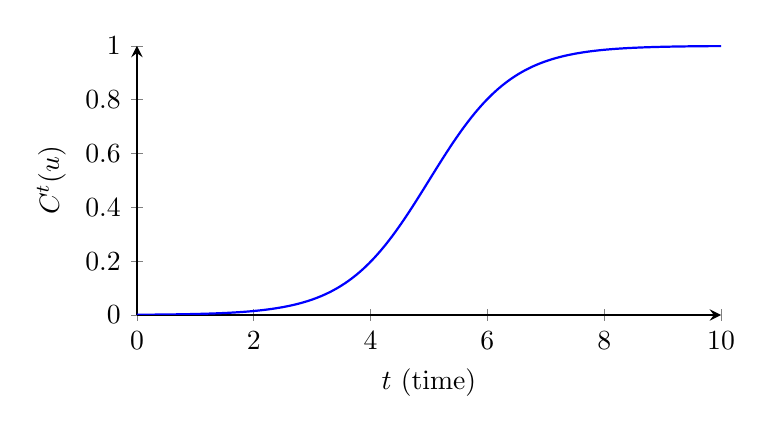
\begin{tikzpicture}
    \begin{axis}[
        width=9cm,height=5cm,
        xlabel={$t$ (time)},
        ylabel={$C^{t}(u)$},
        ymin=0, ymax=1,
        domain=0:10, samples=200,
        axis lines=left, thick]
      \addplot+[no marks] {1 / (1 + exp(-1.4*(x-5)))}; % logistic curve
    \end{axis}
  \end{tikzpicture}
  \caption{Trajectory of community entrenchment
           ($C^{t}(u)$) predicted by the logistic model.}
  \label{fig:trajectory}
\end{figure}


\subsection{Bootstrapping Novel Constructions}

For previously unseen constructions, initial entrenchment is estimated through structural similarity:

\[
C^0(u_{\text{novel}}) = \max_{u' \in \text{Entrenched}} \left[ C^t(u') \cdot \exp(-d(u_{\text{novel}}, u')) \right]
\]
where $d(\cdot, \cdot)$ is a distance metric in feature space (e.g., edit distance over dependency structures). This allows the model to make predictions about novel constructions based on analogical reasoning.

\subsection{Empirical Predictions}

This formalization generates testable predictions:

\begin{enumerate}
    \item \textbf{Measurement convergence}: The indicators $A(u)$, $E(u)$, $P(u)$, and $S(u)$ should load positively on a common factor identifiable as $C^t(u)$.
    
    \item \textbf{Dissociation of frequency and entrenchment}: High $E(u)$ with systematic error properties should predict low $C^t(u)$ and continued ungrammaticality judgments.
    
    \item \textbf{Time-lagged prediction}: Current values of $C^t(u)$ and $\Delta(u)$ should predict future grammaticality judgments according to the logistic growth model.
    
    \item \textbf{Satiation effects}: Experimental manipulation of $E(u)$ should increase $C^t(u)$ only for constructions where NoisePenalty$(u)$ is low.
    
    \item \textbf{Cross-linguistic consistency}: Constructions with similar values of $K(u)$ and $C^t(u)$ should show comparable acceptability across languages, controlling for structural differences.
\end{enumerate}

\subsection{Model Fitting and Validation}

The model parameters can be estimated using hierarchical Bayesian methods:

\begin{enumerate}
    \item Estimate $C^t(u)$ for a sample of constructions using confirmatory factor analysis on the four indicators
    \item Fit the logistic growth parameters using historical corpus data
    \item Validate predictions on held-out constructions and future time points
    \item Compare model predictions to simpler alternatives (e.g., frequency-only models)
\end{enumerate}

This approach transforms the framework from a descriptive theory into a quantitative model capable of precise predictions about grammaticality judgments and their evolution over time.


\section{The Operationalization of \texorpdfstring{$F(u)$}{F(u)}}
\label{sec:Fu}

%-------------------------
\subsection{Definition}
The variable $F(u)\in[-1,0]$ represents the \textit{felt} well-formedness of an
utterance.\footnote{Negative scale is chosen for algebraic symmetry with the
loss terms in §\ref{sec:formalism}; any monotone rescaling would be equivalent.}
It is computed at the output of comprehension, not during
incremental parsing:

\[
F(u)=
 -\alpha\bigl(1-G(u)\bigr)
 -\beta P(u)
 -\gamma D(u)
 +\varepsilon_{\!\text{indiv}} ,
\]

\begin{itemize}
  \item $G(u)\in\{0,1\}$ — objective grammaticality (§\ref{sec:formalism}).
  \item $P(u)\in[0,\infty)$ — residual processing cost after noise filtering
        (surprisal, interference, locality), normalised by the speaker’s
        working-memory span.
  \item $D(u)\in[0,1]$ — degree of prescriptive dissonance: the learner’s
        stored school rules conflicting with the heard form.
  \item $\varepsilon_{\!\text{indiv}}\sim\mathcal N(0,\sigma^2)$ — stable
        speaker-specific bias.
\end{itemize}

%-------------------------
\subsection{Interpretation}
\begin{enumerate}
\item $F(u)=0$ corresponds to a \emph{null affect}: speakers report no
  anomaly. There is no positive hedonic “ah, grammatical!” signal.
\item $F(u)<0$ is a metacognitive warning proportional to the summed evidence
  that something has mis-fired—structurally, procedurally, or socially.
\item The same $F$ value can arise from different mixtures of causes; only the
  decomposition pins down which component(s) are responsible.
\end{enumerate}

%-------------------------
\subsection{Measurement strategy}
\begin{itemize}
  \item \textbf{Explicit ratings}\,: map 7-point Likert or magnitude-estimation
        scores linearly onto $[-1,0]$.
  \item \textbf{Implicit probes}\,: centre-surprisal ERP (N400/P600) and
        self-paced reading slow-downs give continuous proxies for $P(u)$; these
        enter the model as observed covariates when $F$ is treated as latent.
  \item \textbf{Prescriptive load}\,: questionnaire-based index of rule
        internalisation supplies $D(u)$ per participant.
\end{itemize}

%-------------------------
\subsection{Psychometric model}
Let $y_{ij}$ be judge $i$’s rating of item $j$.  
A two-level graded-response IRT model (cf. \parencite{samejima1997}) links the
latent feeling to responses:\footnote{Here $\mathrm{P}$ denotes probability; do not confuse with the processing-cost term $P(u)$.}

\[
\mathrm{P}\!\bigl(y_{ij}\le k \mid F_{ij}\bigr)=
      \bigl[1+\exp\bigl(-a_k(F_{ij}-b_k)\bigr)\bigr]^{-1},
\quad
F_{ij}=F(u_j)+\varepsilon_{\!\text{parsing},ij}.
\]
Disentangling $F$ from $\varepsilon_{\!\text{parsing}}$ recovers the true
latent continuum on which factor analysis (as in § 1) operates.

%-------------------------
\subsection{Functional consequences}
\begin{enumerate}
\item Factor analyses over raw ratings \emph{necessarily} return the structure
      of $F$, not $G$.  Interpret latent dimensions accordingly.
\item Any experiment that manipulates familiarity, working-memory load,
      or prescriptive priming will shift $F$ without changing $G$.
\item In change-over-time studies, $F$ is the leading indicator: entrenchment
      first dampens $\beta P(u)$, then lifts $C^t$ and flips $G$ from $0$ to~$1$.
\end{enumerate}



\section{Theoretical Implications}\label{sec:implications}

MMMG yields several important implications for our understanding of grammaticality:

First, it supports treating grammaticality as an emergent property unified by the stability of form--meaning pairings. Different patterns in the distribution of grammatical constructions across adjective types illustrate this~-- despite the existence of clear patterns governing modifier selection by adjectives, these patterns resist reduction to simple rules. Instead, they arise from complex interactions between modifier semantics, adjective scale structure, and discourse-pragmatic factors. For instance, the distribution of \textit{much} versus \textit{more} with different adjective classes (comparative governors, participial adjectives, etc.) shows complex patterns that can be explained but not easily predicted from simpler principles \autocite{reynolds2024why}. This helps explain why efforts to reduce grammaticality to simple necessary and sufficient conditions have repeatedly fallen short.

Second, this framework clarifies how formal and usage-based approaches capture different aspects of grammatical stability. The stability of grammatical patterns depends both on their internal systematic properties (emphasized by formal approaches) and on their role in meeting communicative needs (emphasized by functional accounts). Many grammatical phenomena exhibit stability patterns that can't be reduced to local collections of features. Consider how discourse context affects grammaticality judgments: whether a construction maintains stable form--meaning relationships often depends on broader patterns of language use that can't be localized to specific morphosyntactic features. This helps explain why purely local syntactic models often fail to capture the full range of grammaticality phenomena.

Third, the analysis suggests specific predictions about how grammatical stability is maintained and lost. If grammatical constructions are maintained through multiple interacting factors, we should expect:
\begin{enumerate}
    \item Instability to manifest in coordinated ways across multiple properties rather than through isolated changes
    \item Periods of gradually increasing instability followed by relatively rapid reorganization when stability thresholds are crossed
    \item Different but equally stable grammatical patterns emerging in different language communities
    \item Gradient effects in grammaticality judgments reflecting varying degrees of stability
\end{enumerate}

Fourth, MMMG illuminates the relationship between competence and performance. Rather than treating these as fundamentally different phenomena, we can understand them as different manifestations of the same stability conditions. Processing limitations and other performance factors help shape which form--meaning pairings become stable, while those stable pairings in turn constrain possible performance patterns.

Finally, this approach offers a new perspective on systematic constraints in grammar, such as the English ban on left-branch extraction. Instead of viewing these as either innate rules or processing limitations, we can understand them as particularly robust stability conditions in form--meaning pairings. Their persistence reflects deep patterns of stability, while cross-linguistic variation shows how different stable solutions can emerge in different communities.

These implications suggest concrete directions for future research. We need more detailed studies of how multiple properties interact to create and maintain stable form--meaning pairings, better methods for measuring degrees of stability, and closer examination of the transition points where grammatical systems reorganize. The framework also calls for renewed attention to variation across language communities, as different stability patterns may shed light on the fundamental nature of grammatical organization.

The crucial idea is that grammaticality represents a real linguistic kind~-- stable form--meaning pairings maintained through community practice~-- rather than merely a disjunctive collection of sufficient conditions. This unifying concept helps explain both the diversity of grammatical phenomena and their underlying commonality.

\subsection{Actuation and the dynamics of grammatical change}

The formal framework developed in \S\ref{sec:formalism} yields important implications for understanding when and why grammatical norms shift within speech communities. The concept of \textit{actuation}~-- the moment when community dynamics shift to favour a linguistic innovation~-- can now be defined precisely as the point when $\Delta = \alpha - \beta$ crosses zero, transforming a construction's status from systematically rejected ($\Delta < 0$) to potentially accepted ($\Delta > 0$).

This bifurcation represents a qualitative change in the community's linguistic system: what was previously a stable equilibrium at $C^t(u) = 0$ (universal rejection) becomes unstable, allowing the construction to spread through the population. The framework thus provides a principled explanation for why certain innovations succeed whilst others fail, even when both appear individually sensible or useful.

The factors that drive such bifurcations align with the motivations discussed in \S\ref{sec:motivations}. Semantic reanalysis may increase $\alpha$ by making a form--meaning pairing more transparent or useful. Social pressures may simultaneously increase $\alpha$ (through prestige effects) and decrease $\beta$ (by reducing resistance to the innovation). Structural motivations such as analogical extension can systematically raise $\alpha$ by providing speakers with familiar patterns to guide their acceptance. Processing constraints may affect both parameters: forms that become easier to parse see increased $\alpha$, whilst those that strain cognitive resources face elevated $\beta$.

Actuation is not simply a matter of individual innovation but requires coordinated community-level change. A few speakers adopting a marginal construction does not guarantee its success; actuation demands that the underlying dynamics shift such that acceptance systematically outweighs rejection across the speech community. This explains why many innovations fail despite being individually sensible~-- they appear before the community conditions are right for $\Delta$ to become positive.

The bifurcation framework also clarifies why certain changes appear to accelerate once they begin. Near the critical point $\Delta = 0$, small perturbations in community attitudes can trigger rapid shifts between rejection and acceptance. As $\Delta$ becomes more strongly positive, the construction moves further from the unstable rejection state, making reversal increasingly unlikely. This creates the characteristic S-curve pattern observed in many documented language changes~\autocite{kroch1989}, emerging naturally from the underlying population dynamics.

For constructions currently existing in the marginal zone~-- those with $\Delta \approx 0$~-- the framework predicts heightened sensitivity to external factors and greater cross-community variation. Small speech communities may show particularly volatile behaviour near bifurcation points, as stochastic effects can overwhelm weak deterministic trends. This may explain why certain changes appear to originate in geographically or socially peripheral communities before spreading to larger population centres.

\subsection{Relationship to Generative Grammar}

The generative tradition has provided linguistics with foundational contributions into the systematic nature of grammatical knowledge. Most fundamentally, it demonstrates that grammaticality can't be reduced to semantic plausibility, processing ease, or frequency of attestation. When Chomsky introduced \textit{Colorless green ideas sleep furiously}, he showed definitively that speakers can recognize syntactically well-formed sentences even when they are semantically bizarre. The framework coherently explains categorical constraints like the impossibility of extracting determiner-adjective sequences in English (*\textit{Which do you prefer car?}), and critically, it captures the fact that such sequences remain ungrammatical even when their intended meaning is clear and processing demands are low. 

MMMG shares with generative grammar several foundational observations: that grammaticality judgments reflect systematic, real patterns \autocite{Dennett1991}; that these patterns can't be reduced to meaning or processing alone; and that certain syntactic configurations appear to be categorically excluded regardless of context. The analysis of multiple center embeddings presented in \S\ref{sec:processing} builds directly on ideas about recursive structure, and our treatment of systematic blocking (\S\ref{sec:systematic-blocking}) acknowledges the generative discovery that some constructions appear to be universally excluded by the grammar itself.

The generative tradition has also identified fascinating puzzles that any theory of grammar must address, such as the independent relative \textit{whose} (\ref{ex:whose}). As \textcite{hankamer1973whose} observe, this construction appears to violate no syntactic principles: independent genitives are possible (\textit{Mine was visiting}), independent interrogative \textit{whose} is grammatical (\textit{Whose was open?}), and \textit{whose} functions perfectly well as a dependent relative pronoun (\textit{the student whose friend was visiting}). The generative tradition's careful documentation of such cases, where seemingly parallel constructions show puzzlingly different grammatical status, has been invaluable in pushing theoretical development forward.

Where MMMG departs from generative grammar is in its explanation of such patterns. Rather than positing an autonomous syntactic component, MMMG suggests that grammatical constraints emerge from the interaction of form--meaning pairings within specific language communities and situations. The independent relative \textit{whose} construction illustrates this difference. For this construction to be felicitous, multiple conditions must converge: the possessor must be sufficiently accessible in the discourse while the possessum is predictable enough to license ellipsis, yet the possessive relationship needs to be semantically significant enough to warrant explicit marking. Moreover, this configuration must occur in a context where a relative clause is the optimal way to package this information. The extreme rarity of contexts satisfying all these conditions appears to prevent the construction from becoming conventionalized in the grammar at all~-- speakers encounter it so rarely, despite perfectly common components, that even when all conditions align perfectly, the construction feels alien.

This approach draws on the generative observations about systematic constraints while providing a different perspective on their source. Where generative theory must explain why a syntactically possible and pragmatically useful construction is systematically avoided, MMMG suggests that extreme mismatches between predicted and observed frequency may themselves be evidence of grammatical blocking, even when the exact nature of the block remains unclear. The framework thus preserves what is most valuable in generative theory~-- its recognition of systematic grammatical constraints~-- while embedding those insights in a broader theory of how form--meaning pairings become established and maintained in language communities.

Other cases that generative grammar struggles to explain are those that are grammatical with one meaning but ungrammatical with another, such as (\ref{ex:have-years}) \textit{I have 16 years}. While syntactically identical to grammatical expressions like \textit{I have 16 dollars}, this construction becomes ungrammatical specifically when used to express age. A purely syntactic account must somehow explain why the same structure is well-formed in one case but ill-formed in another, despite no apparent syntactic differences. MMMG, in contrast, locates the source of ungrammaticality in the community's form--meaning conventions: \textit{have}+numeral years has become conventionalized for expressing duration or future time (\textit{I have 16 years until retirement}) but blocked for expressing age, where a different construction (\textit{I am 16 years old}) is the established pattern. Similar cases arise with plural forms that are grammatical with some meanings but not others (e.g., \textit{peoples} for ethnic groups but not multiple individuals) and with verbs that resist certain arguments despite no obvious syntactic prohibition (e.g., \textit{discuss about}). These meaning-dependent grammaticality patterns suggest that what gets blocked or licensed often depends on specific form--meaning associations rather than purely structural constraints.

\subsection{Relationship to Construction Grammar}

Construction Grammar (CxG) \autocite{fillmore1988mechanisms, kay1999grammatical,  goldberg1995constructions, goldberg2019, sag2012sign} represents a significant theoretical advancs in our understanding of linguistic knowledge. At its core, CxG argues that language consists of learned pairings between form and meaning at multiple levels of complexity. These form--meaning pairings, or constructions, range from individual morphemes to abstract syntactic patterns. This perspective helps explain phenomena that proved challenging for earlier approaches, which often struggled to account for how speakers learn and use both regular patterns and idiomatic expressions without requiring separate mechanisms for ``core'' grammar versus ``periphery''.

CxG's most valuable contribution lies in demonstrating that meaning suffuses all levels of grammatical organization. Rather than treating syntax as an autonomous formal system that interfaces with semantics only at certain designated points, CxG reveals how meaning and form are inseparable aspects of linguistic knowledge. For instance, the \textit{What's} X \textit{doing} Y? construction (as in \textit{What's this fly doing in my soup?}) carries an implication of incongruity that can't be derived from its component parts \autocite{kay1999grammatical}. Such examples provide compelling evidence that constructional meaning exists beyond pure compositionality and that constructions inherently package form and meaning together.

Recent work strengthens the empirical foundation for CxG's framework. \textcite{weissweiler2023construction} demonstrate how construction grammar provides a theoretical framework for probing how neural language models handle different levels of linguistic abstraction. Their findings suggest that transformer models may learn construction-like representations, offering new evidence for CxG's cognitive reality while also providing tools for analyzing artificial neural networks.

MMMG shares these fundamental CxG views about the centrality of form--meaning pairings and the importance of treating meaning as integral to grammar rather than merely interfacing with it. But MMMG departs from CxG on at least one key point: while CxG treats all constructions as instances of the same theoretical kind, differing only in their internal complexity and degree of schematicity, MMMG maintains that morphosyntactic form--meaning pairings play a uniquely privileged role in grammaticality judgments.

This difference becomes clear when we account for how speakers judge various types of linguistic violations. While CxG's unified treatment of constructions suggests no principled basis for treating different types of violations differently, speakers consistently judge morphosyntactic violations (like \textit{*Furiously sleep ideas green colorless}) as ``ungrammatical'' in a qualitatively different way than they judge violations of register, politeness norms, or genre expectations. Even when morphosyntactic violations result in perfectly interpretable utterances (like \textit{*I have 25 years} to express age), speakers treat them as ungrammatical in a way that differs from their reactions to pragmatically inappropriate but grammatically stable expressions.

This asymmetry suggests that morphosyntax constitutes a distinct type of linguistic knowledge~-- not because it operates autonomously from meaning (as earlier formal theories claimed), but because it represents a particular kind of form--meaning pairing that plays a special role in defining the basic combinatorial possibilities of a language. MMMG thus preserves CxG's fundamental ideas about the inseparability of form and meaning while recognizing the unique status of morphosyntactic form--meaning pairings in speakers' grammatical knowledge.

By maintaining this position, MMMG captures what is most valuable in the CxG approach~-- its systematic treatment of form--meaning pairings across different levels of linguistic structure~-- while better accounting for the special status that speakers accord to morphosyntactic form--meaning pairings in their grammaticality judgments. Rather than treating this special status as evidence for autonomous syntax (as generative approaches do), MMMG suggests it reflects the unique role that morphosyntactic patterns play in establishing the basic meaning-making resources of a language community.

\subsection{Relationship to Usage-Based Approaches}

MMMG shares with Usage-Based approaches (UBA) \autocite{bybee2006, bybee2007frequency, bybee2010} the idea that linguistic knowledge emerges from patterns of actual language use rather than from an autonomous formal system. Both perspectives reject the notion that grammaticality can be reduced to abstract rules operating independently of meaning and context. However, MMMG diverges from UBA in its treatment of the special status of morphosyntactic well-formedness, particularly in cases where frequency patterns present theoretical puzzles.

The analysis of independent relative \textit{whose}, as in \textsuperscript{?}\textit{I saw Joan, a friend of whose was visiting} is a case in point. A simple UBA account might predict that this construction's marginality stems from its low frequency. But this explanation proves insufficient: the construction isn't merely rare but dramatically rarer than we would expect given the frequency of its component parts. Independent \textit{whose} appears in interrogatives (\textit{Whose is that?}), and the relative \textit{whose} is common in dependent contexts (\textit{the student whose paper was late}). Given these frequencies, analogical extension should make the independent relative use more common than it is. The extreme rarity of independent relative \textit{whose} in corpora, despite the grammatical availability of comparable elements and contexts, marks it as more than just infrequent~-- it points to a systematic gap in form--meaning pairings.

Where UBA would treat all linguistic patterns~-- whether phonological, morphological, syntactic, or pragmatic~-- as equally driven by usage and frequency effects, MMMG maintains that morphosyntactic patterns play a uniquely central role in grammaticality judgments. This helps explain why some extremely rare constructions remain fully grammatical (like center-embedded relatives), while other constructions that should be analogically available remain stubbornly marginal despite clear communicative potential. The framework suggests that what appears to be simple rarity may sometimes reflect deeper incompatibilities in form--meaning mapping that resist entrenchment even when analogical patterns would predict otherwise.

This theoretical position allows MMMG to incorporate many valuable findings from UBA~-- particularly regarding the role of frequency in entrenching constructional patterns~-- while maintaining crucial distinctions between morphosyntactic well-formedness and other types of linguistic acceptability. Cases like independent relative \textit{whose} demonstrate that we need a theory that can distinguish between patterns that are simply uncommon and those that are systematically excluded from the grammar in ways that resist frequency-based explanation.

\subsection{Relationship to Logicality of Language Accounts}

An alternative perspective, prominent in recent formal semantics, suggests certain types of unacceptability stem from the language faculty itself possessing a deductive system that identifies and filters sentences with logically trivial meanings (tautologies or contradictions) \autocite[cf.][]{del_pinal_logicality_2019, chierchia_logic_2013, fox_economy_2000}. This `logicality of language' hypothesis attempts to explain, for example, systematic restrictions on quantifiers by arguing the unacceptable cases are `L-trivial'~-- their triviality arises solely from the meaning and configuration of logical/functional terms (like \textit{every}, \textit{some}, \textit{not}), irrespective of the open-class words (like \textit{student}, \textit{run}) \autocite{gajewski_l-triviality_2009}. A key challenge is explaining why simple tautologies or contradictions (e.g., \textit{It is raining and it is not raining}) are often acceptable. \textcite{del_pinal_logicality_2019} argues against `Logical Skeletons' (which assume the system ignores open-class word identity) in favour of `LF+RESCALE', a view where the system sees standard logical forms but allows optional, context-dependent modulation of open-class terms (e.g., interpreting the second `raining' as `raining hard') to yield non-trivial meanings.

MMMG offers a potentially broader and more unified account. While `logicality' approaches excel at explaining restrictions tied to functional vocabulary via L-triviality, MMMG aims to cover a wider spectrum of ungrammaticality, including cases not easily reducible to logical contradiction, such as absent form--meaning pairings (\ref{ex:nonsense}), strong deviations from conventional community forms (\ref{ex:sheeps}), or extreme, unexpected rarity (\ref{ex:whose}). Furthermore, by grounding grammaticality in community-specific conventions (\S\ref{sec:f-m-pair-in-community}) and allowing for gradient compatibility ($K(u)$) and acceptance ($C^t(u)$), MMMG inherently accommodates cross-linguistic variation and degrees of acceptability, aspects less central to the L-triviality filter. While LF+RESCALE provides a specific mechanism for acceptable `trivialities', MMMG suggests these might arise from more general principles of interpretation within community norms, potentially avoiding the need to posit a dedicated deductive module and specific operators like RESCALE, and offering a clearer distinction between objective grammatical status and subjective processing effects or `feelings' (\S\ref{sec:feeling}). Thus, MMMG frames grammaticality as an emergent consequence of communicative practice rather than a direct output of logical computation within syntax.



\subsection{Relationship to Relevance-Theoretic Accounts}

Recent work by \textcite{scottphillips2024communication} offers a fundamental observation: linguistic intuitions about acceptability arise as byproduct effects of our cognitive systems for interpreting communicative acts. Just as we immediately sense when a visual stimulus violates core assumptions about physical objects (as with impossible objects), we detect when utterances violate basic presumptions about communicative efficiency. Significantly, Scott-Phillips argues that unacceptability occurs not from mere inefficiency, but from an inherent impossibility of interpreting an utterance consistently with these presumptions~-- similar to how an impossible trident (Figure \ref{fig:impossible trident}) can't be interpreted as physically cohesive in any context.

\begin{figure}
    \centering
    
\includegraphics[width=0.2\linewidth]{trident.jpg}
    \caption{Impossible trident}
    \label{fig:impossible trident}
\end{figure}

MMMG shares several key premises with this account. Both frameworks reject the need for an innate grammar faculty, locating linguistic intuitions instead within general cognitive systems. Both recognize that language emerges from communicative needs rather than autonomous syntactic principles. MMMG's emphasis on community-specific form--meaning pairings builds directly on Scott-Phillips's arguments about how communicative pressures shape linguistic conventions.

The frameworks differ primarily in their explanatory mechanisms. Where Scott-Phillips argues that grammaticality judgments reduce to impossibilities of efficient interpretation, MMMG suggests that while communicative pressures shape which form--meaning pairings become conventionalized, these pairings then create systematic constraints that can't be reduced to efficiency alone. For Scott-Phillips, we must demonstrate that (\ref{ex:tense}) contains inherent contradictions making efficient interpretation impossible. MMMG instead analyzes how the meaning of tense--aspect morphosyntax clashes with the meaning of the lexeme \textit{yesterday}. While these analyses might ultimately converge, it remains unclear why the criterion of inherent impossibility of interpretation should apply specifically to morphosyntactic violations rather than to lexical-lexical conflicts or certain phonological patterns. The scope of what constitutes an interpretive impossibility requires further theoretical development.

This difference has important empirical implications. MMMG makes relatively concrete demands: we can test whether specific form--meaning pairings are stable within a community and identify precise points of morphosyntactic-lexical conflict. The challenge for relevance-theoretic accounts, as Scott-Phillips (personal communication, Dec. 16, 2024) acknowledges, lies in establishing independent, empirically vulnerable claims about what makes efficient interpretation inherently impossible rather than merely difficult. Future work comparing specific predictions of each approach~-- particularly around how novel constructions become acceptable or unacceptable~-- could help clarify their relationship and complementary insights.

\subsection{Predictions}

This framework predicts that grammaticality judgments will vary systematically across languages depending on the degree to which morphosyntactic and lexical meanings are required to align. A prime example of this variation can be seen in the cross-linguistic treatment of gendered pronouns. In Spanish, grammatical gender permeates the morphosyntactic system, mandating concord across determinatives, adjectives, and nouns. English, in contrast, exhibits a far weaker grammaticalization of gender, primarily restricted to pronoun selection. Japanese, meanwhile, lacks grammatical gender entirely, arguably using a fundamentally different system of person reference; consequently, any notion of gender primarily operates at the lexical or pragmatic level.

These cross-linguistic differences generate specific, testable predictions within the proposed framework.  I predict that Spanish speakers will judge sentences with pronoun-antecedent gender mismatches as strongly ungrammatical, reflecting the obligatory alignment of morphosyntactic and lexical gender in the language. English speakers, though, are predicted to exhibit more gradient judgments, with mismatches perceived as moderately ungrammatical due to the weaker integration of gender into the morphosyntax. Finally, Japanese speakers are expected to show the highest tolerance for such mismatches in their equivalent referential forms, potentially judging them as pragmatically infelicitous rather than grammatically ill-formed, since grammatical gender plays no role in the language.

This paradigm can be extended beyond gender to investigate other grammatical features that exhibit cross-linguistic variation in their degree of morphosyntactic integration. Similar tests could be conducted for phenomena such as number, person, definiteness, tense, aspect, and evidentiality, providing a robust empirical foundation for understanding the interplay between morphosyntactic form, lexical meaning, and the diverse ways in which languages structure grammatical systems.

\bigskip
Another key prediction of this framework is that satiation~-- the phenomenon where repeated exposure to an ungrammatical construction leads to increased acceptability~-- should be readily inducible for many types of ungrammaticality, particularly those involving mismatches between morphosyntactic and lexical meaning or those arising from processing constraints.

For instance, consider the case of the independent relative \textit{whose}, as in \textsuperscript{?}\textit{The packages are still here, but Nathan, whose was open, just left.} While initially judged as ungrammatical by many English speakers, this construction might become more acceptable with repeated exposure to independent relative \textit{whose}. This is because the ungrammaticality likely stems from a combination of factors:

\begin{enumerate}
    \item Low Frequency: Independent relative \textit{whose} is extremely rare, leading to a lack of entrenchment.
    \item Processing Difficulty: The construction may pose a parsing challenge in retrieving the possessum from the context.
    \item Competition with a Preferred Alternative: The more frequent and established construction with the dependent relative pronoun (\textit{whose package was open}) competes with the independent \textit{whose} form.
\end{enumerate}

This multi-factorial analysis of ungrammaticality parallels findings from acquisition research. \textcite{dressler1995} demonstrate that children's early morphological development shows similar interactions between frequency, processing constraints, and competition from established forms. Their work suggests these factors represent general principles in how form--meaning pairings become stabilized or blocked within a community.

According to the framework, repeated exposure could lead to satiation because of:

\begin{enumerate}
    \item Increased Familiarity: Repeated encounters would increase the familiarity of the independent relative \textit{whose} construction.
    \item Reduced Processing Load: With practice, the parsing difficulty associated with the construction might decrease.
    \item Weakening of the Competitor: The dominance of the alternative construction might diminish as the independent \textit{whose} form becomes more entrenched.
\end{enumerate}

Crucially, the framework predicts that satiation will be more likely and more pronounced for constructions where the ungrammaticality is due to factors like low frequency, processing difficulty, or weak morphosyntactic integration, rather than a violation like that imposed by left branch extraction (e.g., *\textit{What did you see car?}).

\bigskip
The MMMG framework also makes specific predictions about second language acquisition. Since grammaticality judgments depend on established form--meaning pairings within a language community, learners encountering a new language should initially perceive it as lacking meaningful structure rather than explicitly ungrammatical. While some meaning may be derived through cognates or gestures, much of the input will appear as ``noise'' due to the absence of shared conventions. As learners begin acquiring basic form--meaning correspondences, they are predicted to show heightened sensitivity to violations, marking as ungrammatical many constructions that native speakers accept. This sensitivity reflects interference from L1 form--meaning pairings and incomplete internalization of L2 norms, both of which contribute to the gradient nature of early L2 grammaticality judgments.

Finally, as learners join the L2 speech community and internalize its form--meaning pairings, their judgments should gradually align with those of competent speakers or signers. This trajectory differs from traditional competence-based accounts, which treat grammaticality as an all-or-nothing property. Instead, the MMMG framework predicts that learners’ judgments will initially be more gradient, reflecting partial integration into multiple linguistic systems. This gradience arises from the competing influences of L1 transfer, incomplete entrenchment of L2 norms, and reduced exposure to native-like input. This view aligns with Selinker's (\citeyear{selinker1972}) concept of interlanguage, which similarly conceptualizes L2 development as involving systematic intermediate states rather than simple progression from ``incorrect'' to ``correct'' grammar.

The prediction of initial ``meaninglessness'' could be tested through psycholinguistic measures, such as ERP studies tracking neural responses to unfamiliar structures or self-paced reading tasks assessing the processing of anomalous input. These methods would provide empirical evidence distinguishing the MMMG framework from traditional SLA models, which emphasize innate competence and static grammaticality judgments. Integrating these predictions with research on interlanguage development and transfer could further refine the framework’s applicability to SLA contexts.

\section{Limitations}\label{sec:limitations}

While the proposed framework offers a comprehensive account of grammaticality, integrating insights from various theoretical traditions, it's not without limitations. One potential limitation lies in the framework's reliance on the concept of ``community''. Defining the boundaries of a linguistic community and determining the precise set of shared norms that govern grammaticality judgments within that community can be challenging. The framework acknowledges the fluidity and heterogeneity of language use, but further research is needed to develop more precise methods for operationalizing the notion of community and measuring its influence on grammatical stability.

Furthermore, the framework, in its current form, may not fully capture the complexities of stylistic variation and individual preferences. While it accounts for broad patterns of acceptability and rejection, it doesn't delve deeply into the nuances of stylistic choices that fall within the realm of grammatical acceptability. Future refinements could incorporate a more fine-grained model of stylistic variation and its interaction with core grammatical principles.

Another potential limitation concerns the framework's ability to account for purely formal constraints that seem to exist independently of meaning or communicative function. While the paper argues that many seemingly arbitrary restrictions can be explained by historical processes and the interplay of various motivations, there may be residual cases of purely formal constraints that resist explanation within the current framework. Further investigation into these cases could lead to a more complete understanding of the factors shaping grammatical systems.

%Finally, the framework's emphasis on the interaction between morphosyntactic form and lexical meaning might not fully extend to phenomena at the phonology--syntax interface. While the paper briefly touches upon the role of phonological factors, a more thorough integration of phonological constraints and their influence on grammaticality judgments would be a valuable addition.

Despite these limitations, the proposed framework provides a robust and flexible foundation for understanding the multifaceted nature of grammaticality. It offers a promising avenue for future research, and the limitations outlined here serve as points of departure for further refinement and elaboration.

%\section{Methodological Considerations for Future Research}\label{sec:Methodological-Considerations}

%The development of experimental syntax since the 2000s \autocite{sprouse2016,schutze2016} has revolutionized how we measure and understand gradient acceptability. These sophisticated methodologies allow researchers to quantify subtle differences in grammaticality judgments and track how these judgments change with exposure. The experimental approach has been particularly valuable in bridging the competence--performance divide established in early generative work, providing empirical evidence for how processing constraints interact with grammatical knowledge.

%The framework’s predictions encourage empirical investigation through corpus-based, experimental, and cross-linguistic studies. Several methodological avenues stand out:

%\begin{enumerate}
%\item \textit{Corpus analysis:} Large, balanced corpora allow researchers to track frequency patterns, stability, and emergent constructions over time. Investigating rare or marginal forms (e.g. the independent relative \textit{whose}) in corpora can reveal whether low frequency corresponds to genuinely unstable morphosyntactic patterns or merely a sampling gap. Comparative corpus research in multiple languages can test predictions about how community values influence grammatical distinctions.

%\item \textit{Grammaticality judgment experiments:} Controlled psycholinguistic tasks, including magnitude estimation or forced-choice paradigms, can assess subtle gradience in grammaticality judgments. By manipulating exposure and increasing familiarity with marginal forms, researchers can measure satiation effects and distinguish between stable categorical blocks and constructions that become more acceptable through repeated exposure.

%\item \textit{Processing measures:} Eye-tracking, self-paced reading, and EEG studies can identify whether some judgments arise from processing overload rather than stable grammatical constraints. If a form becomes easier to parse with practice, it suggests that processing complexity, rather than an immutable rule, lies behind initial judgments of ungrammaticality.

%\item \textit{Sociolinguistic fieldwork:} Investigations in communities with distinct dialects or multilingual practices can clarify how social and pragmatic motivations shape grammatical stability. Elicitation tasks and careful comparisons across speech communities can confirm that what counts as grammatical depends on local norms rather than universal principles.

%\item \textit{Longitudinal and historical studies:} Diachronic corpora and historical grammars can trace how marginal constructions evolve, testing predictions about which factors lead certain patterns to stabilize, which fade, and which undergo reanalysis. Tracking a community’s acceptance of previously dubious constructions over time provides direct evidence for the gradual entrenchment processes posited by the framework.
%\end{enumerate}

\section{Conclusion}

This paper has proposed a novel framework for understanding grammaticality, one that moves beyond the traditional competence-performance dichotomy and embraces the dynamic interplay of form, meaning, processing constraints, and sociolinguistic factors. By conceptualizing grammaticality as an emergent property of stable form--meaning pairings within specific language communities, the framework accounts for both the categorical and gradient aspects of grammaticality judgments. It explains why some constructions are rigidly ungrammatical, others fluctuate between marginal and acceptable, and still others evolve into stable, conventionalized patterns.

The framework's core tenets~-- that grammaticality involves conventional form--meaning pairings, that these pairings interact with processing constraints and sociolinguistic factors, and that different types of violations arise from different mismatches between form and meaning~-- provide a principled basis for understanding a wide range of linguistic phenomena. The analysis of examples drawn from both formal syntax and experimental data has demonstrated the framework's explanatory power, illuminating challenging cases that have resisted unified explanation in previous approaches.

The framework generates testable predictions about which ungrammatical constructions might change over time and offers potential applications for language teaching, clinical linguistics, and language documentation. It predicts that grammaticality judgments will vary systematically across languages depending on the degree of alignment between morphosyntactic form and lexical meaning and that satiation effects should be more readily inducible for constructions where ungrammaticality stems from factors like low frequency, processing difficulty, or weak morphosyntactic integration rather than categorical violations.

Integrating the methodologies outlined in the previous section offers a path toward a more comprehensive understanding of how form--meaning pairings become stable within communities, what factors promote or inhibit their entrenchment, and how cross-linguistic variation arises. Future work can refine the metrics for identifying stable form--meaning mappings, develop computational models to predict emergent regularities, and expand the empirical base to underrepresented languages and language contact situations.

While acknowledging the limitations of the current formulation, this paper argues that the proposed framework represents a significant step toward a more comprehensive and nuanced understanding of grammaticality. By integrating insights from generative, functional, and usage-based approaches, it offers a unified perspective that recognizes the multifaceted nature of linguistic knowledge and its grounding in both individual cognition and community practice.

Future research should focus on further refining the framework, developing more precise methods for measuring form--meaning stability, and investigating the complex interactions between different types of motivations (semantic, social, structural, and iconic). Cross-linguistic studies, particularly those focusing on languages with different degrees of morphosyntactic integration of features like gender, will be important for testing the framework's predictions and exploring the diverse ways in which grammatical systems can emerge and evolve.

Ultimately, the study of grammaticality offers a window into the fundamental workings of human language. By de-idealizing grammaticality and embracing its dynamic, community-relative nature, we can gain a deeper understanding of the cognitive and social forces that shape language. This framework provides a robust foundation for such investigations, paving the way for a more integrated and comprehensive understanding of what it means for an utterance to be considered part of a language.

\newpage
\appendix

\section{Turkish vowel harmony and the morphosyntax--phonology interface}
\label{app:turkish-harmony}

Turkish illustrates a sharp distinction between \emph{lexical} disharmony inside stems and
\emph{allomorphic} harmony on inflectional suffixes.%
\footnote{See \autocite{Sezer1981,KabakVogel2001} for discussion of the phonology and \autocite{Arik2015} for experimental evidence on native judgments.} 
Only the latter interacts with morphosyntactic well‑formedness in the sense of the MMMG.

\paragraph{Stem‑internal vowels: disharmony tolerated.}
Loanwords such as \textit{doktor} `doctor' violate backness harmony, yet are fully acceptable;
the language community simply memorises the form, so $C(u)=1$ and $K(u)=1$.

\ea \label{ex:doktor}
\gll doktor \\
     doctor\\
\glt `doctor' (disharmonic stem, grammatical)
\z
Because no morphosyntactic feature is left unrealised, the morphosyntax--meaning
mapping $\!M(u)\!\rightarrow\!\mu(u)$ succeeds and
\[
G(u)=C^t(u)\cdot K(u)\cdot\text{map}=1.
\]

\paragraph{Suffixal harmony: morphosyntactic requirement.}
Inflectional morphemes are lexicalised with an underspecified vowel;
the correct allomorph must copy \textsc{[±back]} (and, for some
suffixes, \textsc{[±round]}) from the final stem vowel.
Using the ``wrong'' vowel leaves part of the feature bundle unrealised,
so $K(u)=0$ and the word is ungrammatical.

\ea  \label{ex:kitap-pl}
\ea[]{\gll kitap-lar\\
          book-\textsc{pl.back}\\
      \glt `books' (harmonic, grammatical)}
\ex[*]{\gll kitap-ler\\
          book-\textsc{pl.front}\\
      \glt intended `books' (suffix harmony violation)}
\z
\z

\ea \label{ex:gul-past}
\ea[]{\gll gül-dü\\
          laugh-\textsc{pst.front.round}\\
      \glt `s/he laughed' (harmonic, grammatical)}
\ex[*]{\gll gül-du\\
          laugh-\textsc{pst.back.round}\\
      \glt intended `s/he laughed' (suffix harmony violation)}
\z
\z

\paragraph{MMMG account.}
For the ill‑formed *\textit{kitap-ler} and *\textit{gül-du}:

\begin{itemize}
\item \emph{Mapping} succeeds: the plural / past node selects an exponent.
\item \emph{Compatibility} $K(u)=0$: the chosen allomorph fails to realise the
      \textsc{[back]} feature copied from the stem.
\item \emph{Community acceptance} $C^t(u)=1$: every speaker knows how plural
      and past are expressed.
\end{itemize}

Hence $G(u)=0$ and speakers judge the word as categorically wrong, not merely
odd‑sounding.  By contrast, \textit{doktor} in (\ref{ex:doktor}) keeps $K(u)=1$;
harmony is a phonotactic preference that affects only the phonological
well‑formedness component of $F(u)$, not grammaticality.

\paragraph{Localised exceptions.}
Some derivational suffixes (e.g.~\textit{-imsi} `‑ish') are lexically
marked ``disharmonic''.  The community memorises them with $C^t(u)=1$, so no
feature remains unrealised and $G(u)=1$ despite vowel mismatch.  Clitic
boundaries that start a fresh harmony cycle \autocite{KabakVogel2001} are
handled the same way: they satisfy the morphosyntactic mapping and leave
harmony to phonology alone.

In sum, Turkish suffix harmony errors are genuine morphosyntax--phonology
interface violations, making them \emph{ungrammatical} under MMMG, whereas
stem disharmony merely lowers phonological well‑formedness and so affects only
the listener's feeling $F(u)$.



If it could be shown that phonology alone caused feelings of ungrammaticality, that would constitute a serious challenge to this framework's central claim about the necessary involvement of morphosyntactic form--meaning pairings in grammaticality.


\newpage
\section*{Acknowledgements}
Thanks to Peter Evans, Geoff Pullum, Muhammad Ali Khalidi, and Ryan Nefdt, Irene Kosmas, and Mostafa Hasrati for comments and suggestions. I'd like to thank Jamie Ramsden for bringing up the cases of \textit{a orange} and \textit{le hiver}. Henri Kauhanen for reviewing the formalization.

I used the large language models Claude 3.5, ChatGPT o1 pro, and DeepSeek V3 in drafting and editing this paper.

\newpage
\begin{sloppypar}
\printbibliography[title=References]
\end{sloppypar}


\end{document}
